\documentclass{report}
\usepackage[utf8]{inputenc}
\usepackage{times}
\usepackage{cite}
\usepackage{hyperref}
\usepackage{tablefootnote}
\usepackage{graphicx}
\usepackage{float}
\usepackage{listings}
\usepackage{xcolor}
\usepackage{enumitem}
\usepackage{array}

% set the default code style
\lstset{
    frame=tb, % draw a frame at the top and bottom of the code block
    tabsize=4, % tab space width
    showstringspaces=false, % don't mark spaces in strings
    commentstyle=\color{green}, % comment color
    keywordstyle=\color{blue}, % keyword color
    stringstyle=\color{red}, % string color
    basicstyle=\footnotesize
}

\hypersetup{
    colorlinks,
    citecolor=black,
    filecolor=black,
    linkcolor=black,
    urlcolor=black
}

\title{Smartphone App Concept for Medical Applications.}
\author{Alexander Gustafson\\
  University of Applied Sciences,\\
  Zürich,\\
  Switzerland,\\
  alex\_gustafson@yahoo.de}
\date{\parbox{\linewidth}{\centering%
  \today\endgraf\bigskip
  Dozent: Reto Knaack (knaa@zhaw.ch)\endgraf\bigskip
  School of Engineering, Abteilung Zürich \endgraf
  Studiengang Informatik\endgraf
  }}

\begin{document}
\maketitle

\chapter*{Abstract}
The market for smartphone based medical applications is a relatively new and growing quickly. The majority of medical apps are relatively simple health management and tracking applications that might remind a user to take his or her medicine or monitor blood pressure and heart rate data provided by accompanying devices. However, more sophisticated apps can directly provide diagnostic information by capturing and analysing data directly. Several apps exist that can asses the risk of skin cancer by tracking changes in the growth of skin lesions over time.


\tableofcontents

\chapter{Introduction}

\chapter{Project Goals}

\chapter{Market Research}


\section{Data Gathering}

\subsection{Gathering Data from the Apple iTunes Store}

Searching the Apple iTunes store is typically done manually via the iTunes Application from which text and data cannot be automatically extracted. Therefore, searching for and gathering data about IOS Applications is not easy. However, Apple does provide an rss feed that can be used to list Apps in specific categories and ordered according to how new, or how popular they are and if they are free or not. The rss feed is limited to 100 items per category. The data provided by the rss feed is minimal, not much more than title and a text description of the app. There are no sub-genres or tags than can be used to further differentiate the apps.

Using a python script data was gathered from the following rss feeds:

Top 100 Free Medical Apps
Top 100 Grossing Medical Apps
Top 100 Paid Medical Apps
This combined results included data about 255 IOS apps. The title and description fields were imported into a database. Other information from the data such as price, right, or image link were ignored.


\subsection{Gathering App Data from the Google Play Store}

In order to gather data from the Goole app store a script was programmed that could extract lists of apps from a specific url. The following urls were scanned:
\noindent
\begin{itemize}
\item Top Paid Medical Apps : https://play.google.com/store/apps/category/MEDICAL/collection/topselling\_paid

\item Top Free Medical Apps : https://play.google.com/store/apps/category/MEDICAL/collection/topselling\_free
\end{itemize}

For each app listed the script would extract the url of the app's detail page. From the detail page more imformation would be gathered and stored in a database. The data set is similar to that of the itunes rss feed. The title and description text were imported, other fields such as pricing and copyright were ignored.

Data on 480 Medical Apps for Android was imported. However a significant percentage of the apps could not be classified because the description text was in a language other than English, German, or French.


\section{Categorization}

The term "Medical App" is broad and neither the iTunes nor Google app stores offer any kind of sub categorization. In order to get a better overview of what sort of Medical Apps are available it was necessary to manually browse the gathered data and assign categories to the apps.

A database management tool was created using the python based Django Web Framework. Django provides many tools that makes constructing and interacting with databases very easy. The built-in backend administration tool can be configured to browse, edit, and filter data.

In order to quickly browse through and categorize over 700 apps. The Django backend admin was configured so apps could be categorized one after the other with a minimum of clicks or scrolling. The user was presented a list of uncategorized apps. The first one is clicked. The user is then presented with a page displaying the title and summary text of the app and a field from which a category can be selected. Once saved, the app is no longer presented on the list, the user can select the next app at the top of the list.

\subsection{Description of Categories}
\noindent
\begin{itemize}
\item \textbf{Community} - provides some soft of social networking service through which the user can share data with her family or with a network of people suffering from similar disorders.
\item \textbf{Fun / Entertainment} - These apps have to real medical purpose. They are for enjoyment only.
\item \textbf{Alert / First Response} - Apps that assist first responders or that help users alert first responders that help is needed.
\item \textbf{Health / Lifestyle} - Relaxation and meditation apps, or ovulation and fertility reminders
\item \textbf{Resource Finder} - Apps that locate resources in the vicinitly, nearby pharmacies or care providers.
\item \textbf{Reminder} - Apps with timer or calendar functionality that might remind a user of an appointment or manage medince consumption.
\item \textbf{Algorithmic / Diagnostic} - These are apps that provide some sort of diagnositc information based on data that as been gathered by sensors or entered by the user. Examples are seizure detection apps, or stroke severity evalutaion apps.
\item \textbf{Learning / Educational / Reference} - By far the largest category, this includes apps that provide reference information about diseases or education material like anatomy apps for example.
\item \textbf{Organisational} - Apps in this category might help a user or practitioner organise, share or track data and documents. Examples are apps that help users track the status of their blood pressure or blood sugar levels, create health diaries, or manage clinical data and images.
\end{itemize}

\section{Results}


\subsection{IOS Medical Apps}

\begin{figure}[H]
    \centering
    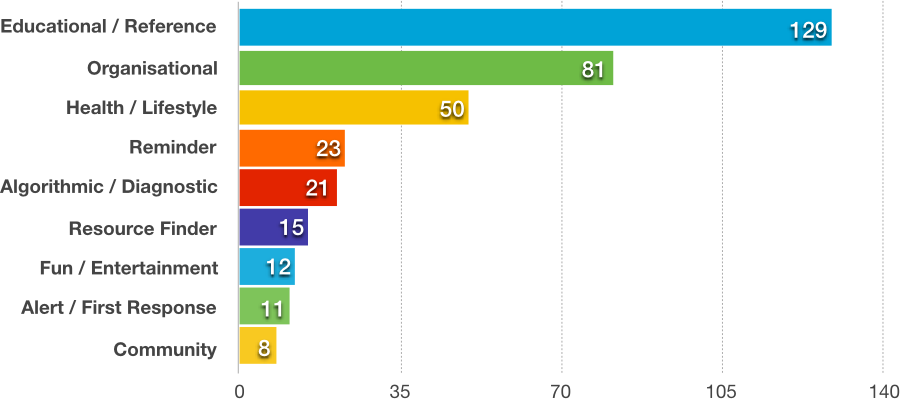
\includegraphics[width=\textwidth]{assets/market_research/apple_chart1.png}
    \caption{Medical Apps on the iTunes Apple Store, Search conducted on 17.05.2016}
    \label{fig:itunes_apps}
\end{figure}


\subsection{Android Medical Apps}

\begin{figure}[H]
    \centering
    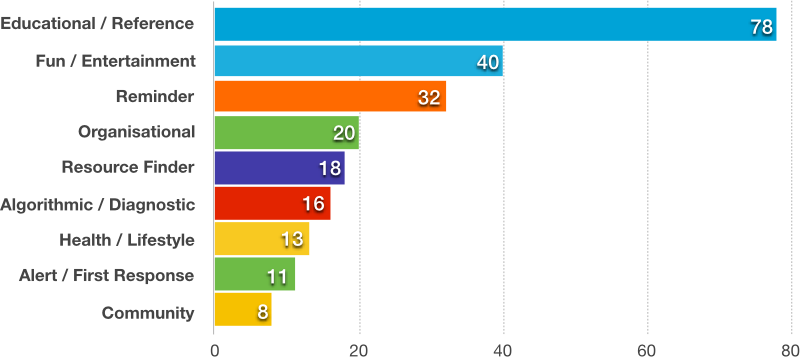
\includegraphics[width=\textwidth]{assets/market_research/android_chart.png}
    \caption{Medical Apps on the Goolge Play Store, Search conducted on 17.05.2016}
    \label{fig:android_apps}
\end{figure}

\subsection{Dermatology Apps 2013 vs 2016}

Mobile apps are an especially good fit for dermatology-related care. Most dermatological conditions are by nature visible. The initial diagnosis and follow up monitoring is mostly done visually. A mobile device with a camera can aid patients and practitioners in the diagnosis of a dermatological condition and tracking it's development. The article Mobile Applications in Dermatology\cite{Brewer_2013} in 2013 identified 229 dermatology-related apps across 5 app platforms ( Android, Apple, Blackberry, Nokia, and Windows ). These were grouped into categories based on their primary functionality. The "Self-surveillance/diagnosis" category was the second largest on the Android and Apple platforms, with 13 and 24 apps respectively.

\begin{figure}[H]
    \centering
    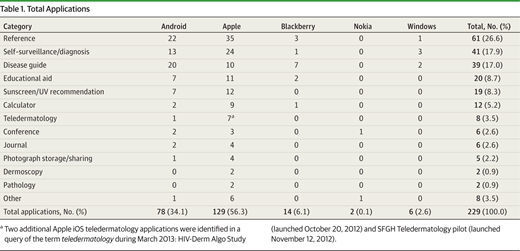
\includegraphics[width=\textwidth]{assets/market_research/brewer.png}
    \caption{Total Applications, Brewer 2013}
    \label{fig:brewer}
\end{figure}

Using the same search criteria and categories from the article above indicates that the availability of dermatological apps is growing. Today there are 33 dermatological apps on the Apple platform that can be identified as having "Self-surveillance/diagnostic" features. With the exception of the "Reference" category, all other categories show significantly higher numbers of available apps.


\begin{figure}[H]
    \centering
    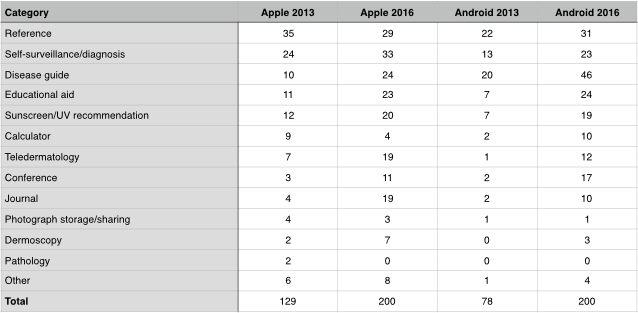
\includegraphics[width=\textwidth]{assets/market_research/apple2013vs2016.png}
    \caption{Demotological Apps by Category, July 2013(Brewer 2013) vs May 2016}
    \label{fig:apps_vs}
\end{figure}

It is important to note that the categories listed above are not defined in the stores. The apps must be manually assigned to a category based on an interpretation of the description text in the store and information obtainable on related websites. It is possible therefore that apps that were originally designated to the “Reference” category might have been interpreted in this paper as a “Educational aid” app for example. The interpretation of the functionality of an app is fuzzy in many cases, and many apps have some crossover functionality. An app developed for self-surveillance will often contain information pertaining to symptoms and treatment ( reference ).

\subsection{Dermatological Apps with Automatic Risk Assesment}

Of the 55 apps identified belonging to the "Self-surveillance/diagnosis" category, only 2 provided risk assesment features based on automatic analysis of captured images.

\noindent
\begin{itemize}
\item SkinVision : https://skinvision.com
\item mSkin Doctor
https://play.google.com/store/apps/details?id=com.maleemtaufiq.mSkinDoctor
\end{itemize}


\chapter{Image Data Sources}
\section{Dermofit}

High quality clinical images with corresponding masks. Great for training and testing.

\begin{table}[H]
\small
    \begin{tabular}{ | l | p{3.5cm} | l | p{3.5cm} |}
    \hline
    Image Type &  Description & Amount & Comment\\ \hline
    Actinic Keratosis &  Pre-cancerous patches of flakey or crusty skin, can develop into Squamous Cell Carcinoma
        & 45 & Not useful as comparison against melanoma \\ \hline
    Basal Cell Carcinoma &  Abnormal, uncontrolled growths of the skin's basal cells.
        & 239 & Not useful as comparison against melanoma \\ \hline
    Dermatofibroma &  Common and benign skin tumour.
        & 65 & Useful as comparison, some extreme cases might have to be left out of the training set. \\ \hline
    Haemangioma &  A collection of small blood vessels that form a lump under the skin.
        & 97 & Useful as comparison, some extreme cases might have to be left out of the training set \\ \hline
    Intraepithelial Carcinoma &  A type of squamous cell skin cancer limited to the upper layer of the skin.
        & 97 & Not useful \\ \hline
    Malignant Melanoma &  A type of cancer that develops from the pigment-containing cells known as melanocytes.
        & 76 & This is our baseline set, half will be used for training, the other half for testing \\ \hline
    Melanocytic Nevus &  Typical mole, benign.
        & 331 & Very usefull as comparison to Melanoma \\ \hline
    Pyogenic Granuloma &  Common skin growth, small, round and red in color due to large number of blood vessels.
        & 24 & Not usefull \\ \hline
    Seborrhoeic Keratosis &  Common non-cancerous skin growth.
        & 257 & Maybe usefull \\ \hline
    Squamous Cell Carcinoma &  Abnormal and uncontrolled growth of squamous cells in the epidermis.
        & 88 & Not usefull \\ \hline

    \end{tabular}

    \caption{Dermofit Image Categories}
    \label{fig:derm_cat}

\end{table}

\section{DermQuest}

Online teaching and learning resource with large image database.

Image were selected based on their usefullness for this project. Usefullness is based on quality and type of image. Dermoscopic images were not selected. Instead images were taken that appeared to be taken with a standard camera. The images only contained the mole to be examined and the surrounding skin area. No other details like eyelids, ears, or dark shadows.

Subgroups of Melanocytic Nevus were chosen. Dysplastic and Intradermal Nevus for the non-cancerous cases, and Malignant Melanoma as the cancerous cases.

\begin{table}[H]
\small
    \begin{tabular}{ | l | p{3.5cm} | l | p{3.5cm} |}
    \hline
    Image Type &  Description & Amount & Comment\\ \hline
    Benign Keratosis &
        & 5 &  \\ \hline
    Malignant Melanoma & A type of cancer that develops from the pigment-containing cells known as melanocytes.
        & 39 & This is our baseline set, half will be used for training, the other half for testing \\ \hline
    Melanocytic Nevus & Typical mole, benign.
        & 51 & Very usefull as comparison to Melanoma \\ \hline

    \end{tabular}

    \caption{DermQuest Image Categories}
    \label{fig:dquest_cat}

\end{table}

\section{PH2Dataset}

Demascopic Images

Many of the mole images extend almost to or even beyond the image border. This makes some of the processing difficult. However the images include an excel spreadsheet which clearly designates what type of mole, including some scoring info such as Asymmetry and Color information.
Includes border mask images.

\begin{table}[H]
\small
    \begin{tabular}{ | l | p{3.5cm} | l | p{3.5cm} |}
    \hline
    Image Type &  Description & Amount & Comment\\ \hline
    Common Nevus &
        & 79 &  \\ \hline
    Atypical Nevus &
        & 79 &  \\ \hline
    Melanoma &
        & 39 & Baseline set for training \\ \hline

    \end{tabular}

    \caption{PH2 Image Categories}
    \label{fig:ph2_cat}

\end{table}

\chapter{TDS Algorithm}
\section{Description of the Algorithm}

Early detection of melanoma greatly increases the chances of successful treatment. A biopsy can be performed in order to gain a definitive diagnosis. However, biopsies are invasive, painful and take time. There are also visual markers Dermatologists look for in order to make a risk assessment. The ABCD Rule, also known as Stokes or TDS Calculation, looks for 4 sets of features. Based on the features the Total Dermoscopy Score (TDS) is calculated.

The 4 sets of features are Asymmetry (A), Border Irregularity (B), Color (C) and Differential Structure or Diameter (D).

Asymmetry can have a value of 0, 1 or 2 depending on the symmetry of the lesion. Where 0 is symmetric and 2 is asymmetric. A value of 1 indicates at least one axis was found across which symmetry exists. The Border score is an integer value from 0 to 8 indicating the presence of border irregularities in 8 regions. Color is an integer value from 1 to 6 indicating the presence of one to six specific colors. Similarly, the value for D indicates the presence of one to five distinct structures or textures. Alternatively, in some literature\cite{Siddiq_2015} D is defined as Diameter, where a diameter greater than 6mm results in a value of 5, otherwise 1.

The final TDS Score is the weighted sum of the ABCD Values and is in the range 1.0 to 8.9.

\begin{equation}
TDS = A * 1.3 + B * 0.1 + C * 0.5 + D * 0.5
\end{equation}

A diagnosis can be made based on the TDS Score according to the following table:

\begin{table}[H]
\centering
\small
    \begin{tabular}{ | l | p{3.5cm} | l | p{3.5cm} |}
    \hline
    Evaluation & TDS Score \\ \hline
    Benign & \textless  4.75  \\ \hline
    Suspicious & 4.75 to 5.45  \\ \hline
    Malignant & \textgreater  5.45  \\ \hline

    \end{tabular}

    \caption{TDS Evaluation\cite{Weigert_2012}}
    \label{fig:tds_eval}

\end{table}


\section{Automatic Calculation of ABCD Values}

The ABCD Rule is used by Dermatologists to differentiate benign from malignant melanocytic tumors. Because it is a clearly defined rule based on easily recognizable visual features it is easy to apply. Clinicians with limited dermoscopy experience achieve better results using the ABCD rule than other methods \cite{Weigert_2012}. The following sections detail methods to automate the calculation of the ABCD scores.

\subsection{Asymmetry}

Asymmetry is a strong indicator of malignancy in a tumor. Of the 4 criteria in the ABCD rule, it is weighted highest.

\subsection{Border}

\subsection{Color}

\subsection{Differential}

\section{Two Examples}
\subsection{Postitiv Example}

\subsection{False Example}

ABCD Values were calculated but classification result was false.

\section{Results of Algorithm}

Performance Evaluation

Chapters 11.1, 11.2, maybe 11.3

\chapter{Image Feature Extraction}
A digital image is a matrix of pixels that contain color information, typically comprised of the 3 color channels red, green, and blue. A person can look at an image and quickly make statements about it's content. For instance, someone might look at an image of a street scene and be able to easily say "This is an image of a street in a town, there is one automobile, three people and a building in this scene". A person would easily be able to draw outlines around the objects and be able to differentiate between areas in each object.

For a computer to be able to "make statements" about the contents of an image it must use algorithms to group together and differentiate between objects in an image. The grouping together and differentiating of areas in an image is known as \textit{segmentation}. The statements that a computer can make about the content of an image are usually of statistical nature and are refered to as \textit{feature extraction}. Before segmentation an image is goes through a \textit{preprocessing} stage in order to remove or reduce irrelevant information or noise.

There are no universal algorithms for preprocessing, segmentation, or feature extraction. The algorithms employed depend on the context of the images to be analyed and the type of information that one is looking for.


\section{Preprocessing}

When capturing an image using a dermatoscope the skin is illuminated equally over the skin area to be photographed. The dermatoscope captures hi-resolution images with low levels of noise. The amount of preprocessing required is limited to colour enhancement to achieve better segmentation results. Using a digital camera like those found in smartphones requires introduces other challenges \cite{auto_seg}.

Unequal illumination or shadows in the image can make it more difficult for the segmentation algorithm to precisely recognise the lesions border. Glare from too much illumination, noise introduced by the circuitry of the sensor in the digital camera or hairs on the skin can also make it difficult to differentiate between the lesion area and healthy skin.

The preprocessing stage attempts to reduce the interference cause by these factors.


\subsection{Equalization}

Histogram Equalisation in image processing is the attempt to enhance detail in images that do not utilise the full range of pixel values. Important details in an image might not be clearly visible because they are is dark areas with low contrast. A histogram of the image is calculated. The histogram shows the distribution of pixels with respect to their brightness or intensity. The intensity of the pixels can be rescaled in order to be evenly distributed.

Depending on the content of an image though global histogram equalisation often makes dark areas darker, light areas become “washed out” and noise becomes more prevalent. This the opposite of what we would like to achieve for dermatological applications. Ideally the healthy skin would be a homogeneous colour and intensity, with no noise or disturbances except for the lesion area to be extracted.

Contrast Limited Adaptive Histogram Equalisation (CLAHE) is an adaptation of Histogram Equalisation but it is not global and it limits the contrast range. CLAHE analyses small regions, or tiles, of the image and enhances the contrast so that the local histogram matches a histogram specified a “Slope” parameter. The tiles are then interpolated together to prevent edge artifacts.

Figures \ref{fig:eq_A} to \ref{fig:eq_C} below show 3 examples of equalised images, comparing the global histogram  equalisation to the CLAHE method.

\begin{figure}[H]
    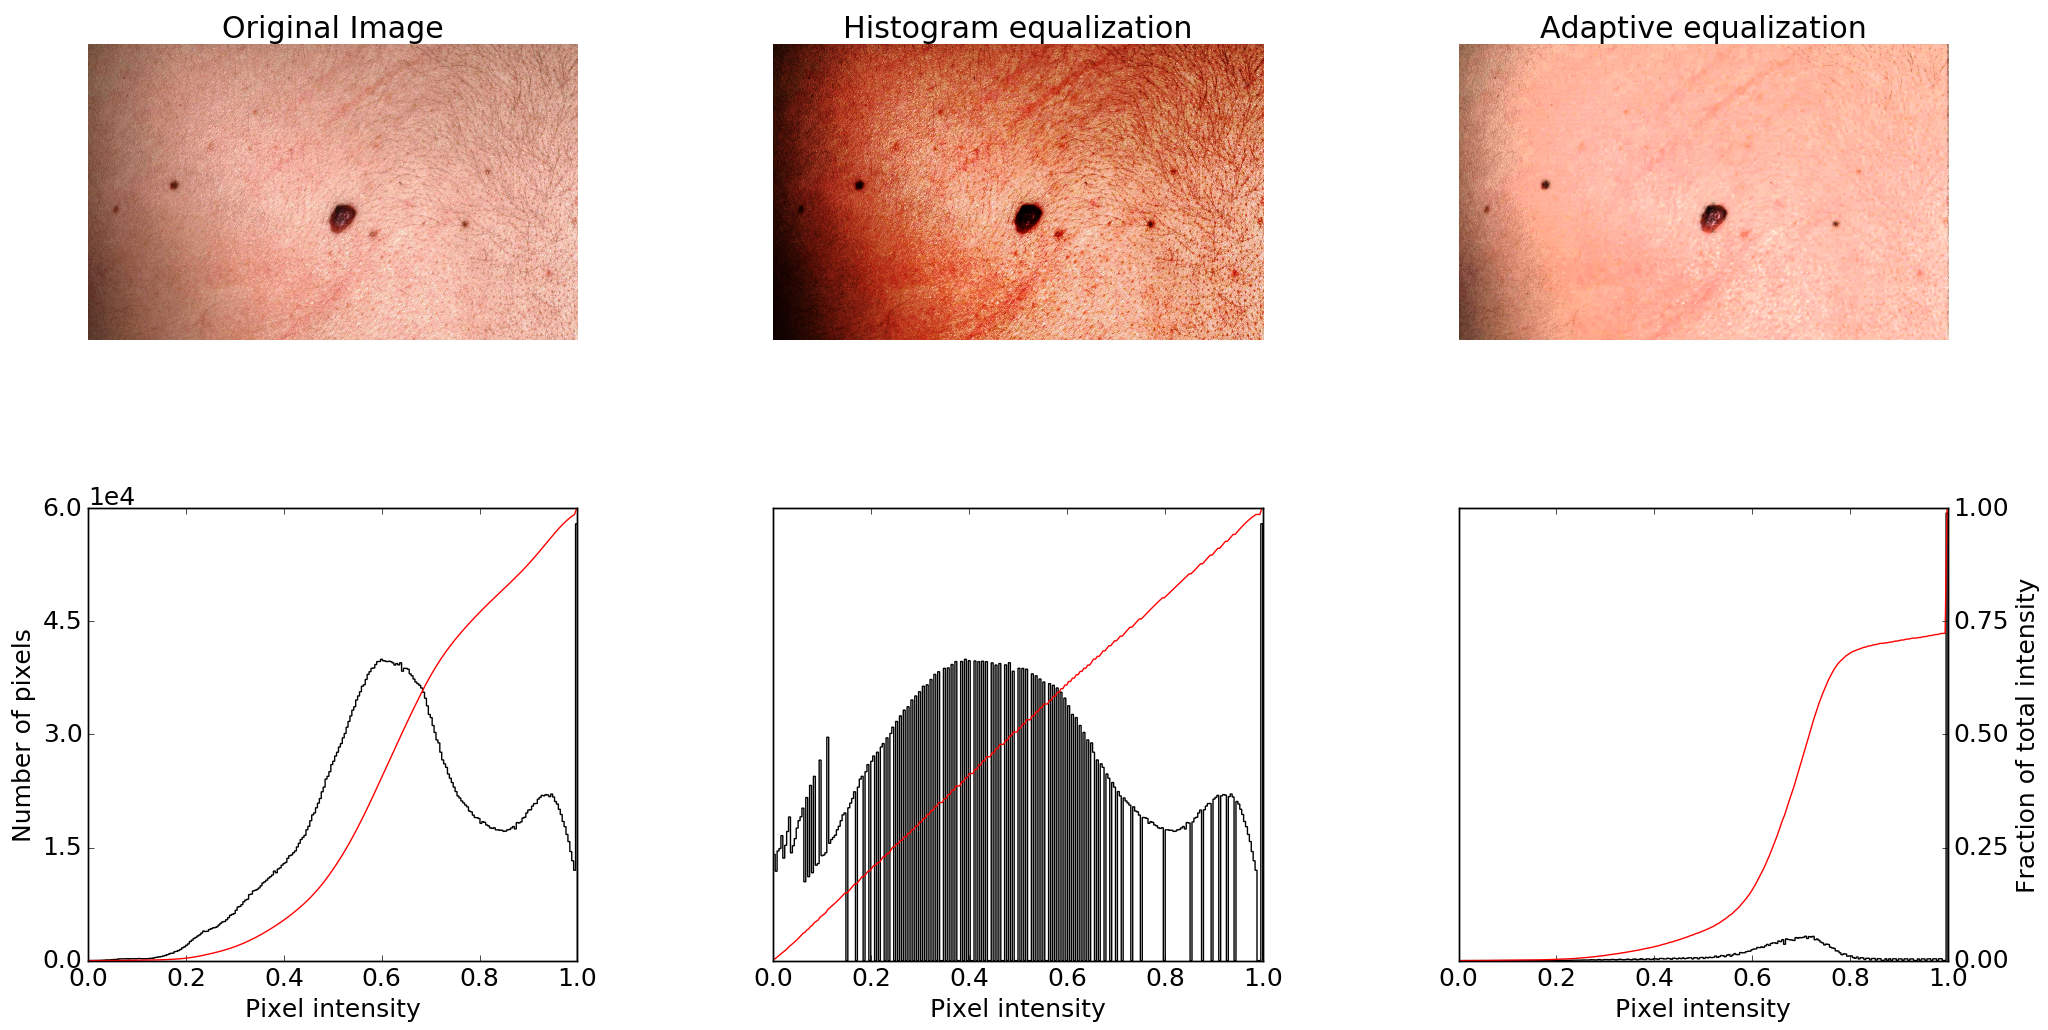
\includegraphics[width=\textwidth,keepaspectratio]{assets/image_processing/equalization/figure_01.png}
    \caption{Image Equalization Example A}
    \label{fig:eq_A}
\end{figure}
\begin{figure}[H]
    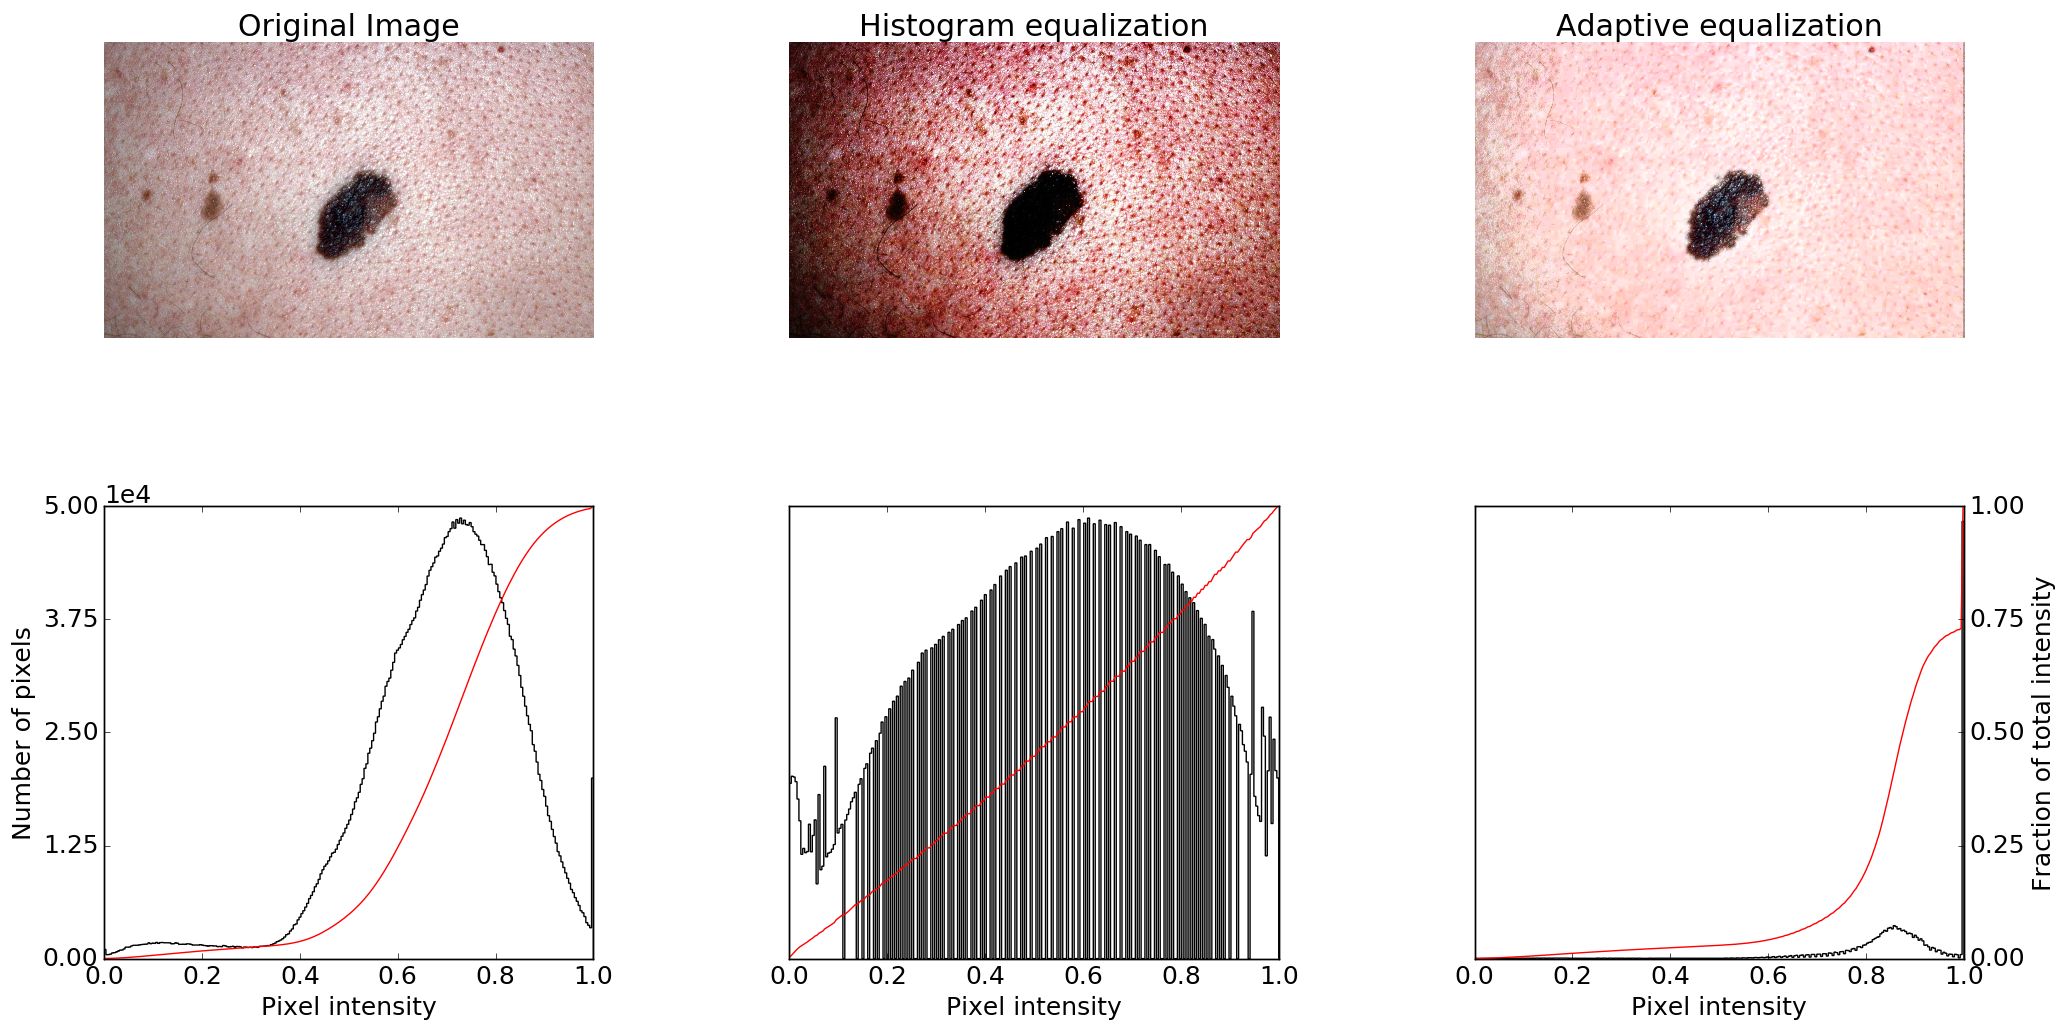
\includegraphics[width=\textwidth,keepaspectratio]{assets/image_processing/equalization/figure_02.png}
    \caption{Image Equalization Example B}
    \label{fig:eq_B}
\end{figure}
\begin{figure}[H]
    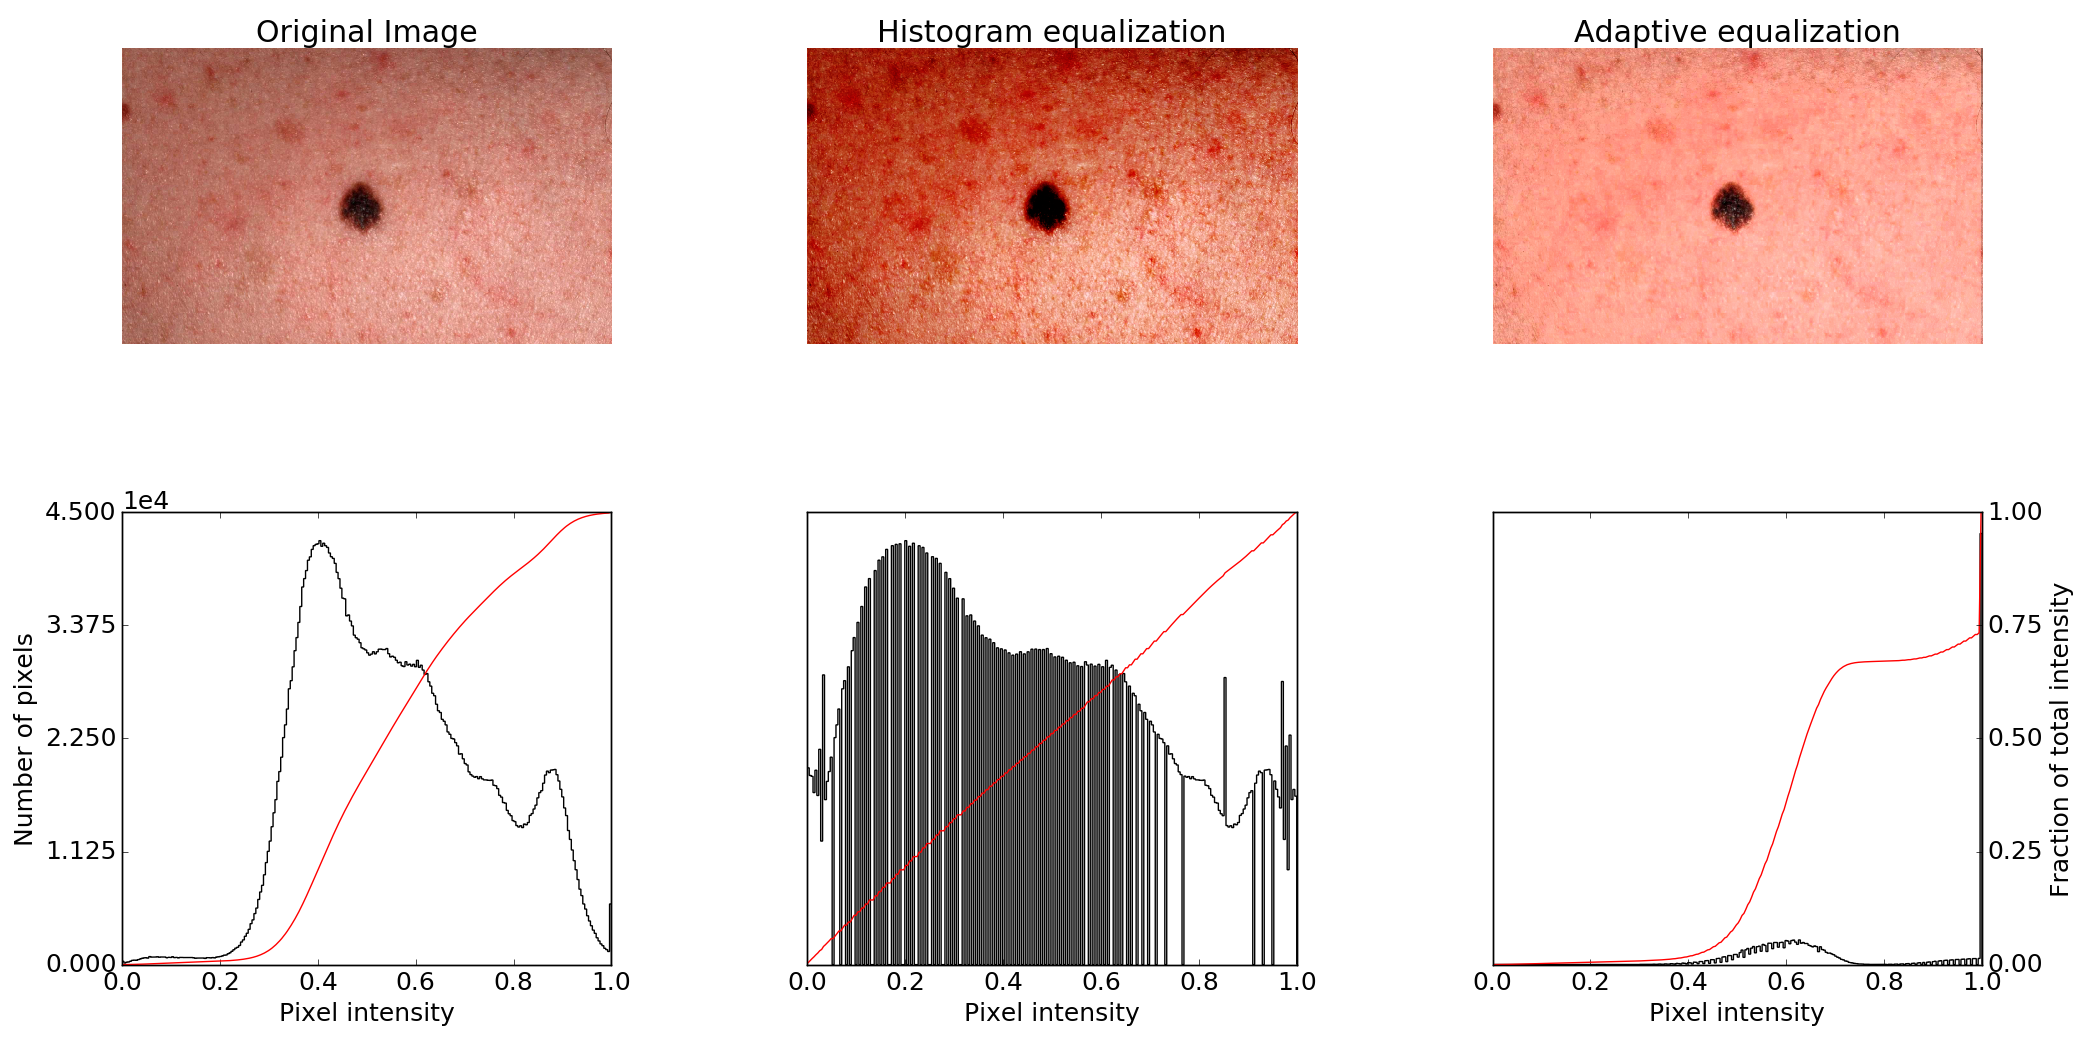
\includegraphics[width=\textwidth,keepaspectratio]{assets/image_processing/equalization/figure_03.png}
    \caption{Image Equalization Example C}
    \label{fig:eq_C}
\end{figure}

\subsection{Noise Reduction}

Noise in a captured image is inevitable, it will be introduced by the circuitry of the camera sensor or even from statistical quantum fluctuations of the photons known as “shot noise” \cite{image_noise}.  Noise in the image produces outlier pixels, pixels that do not represent the surface of the object in the image, and whose values diverge from neighbouring pixels.

Noise in the image will make it more difficult for the segmentation algorithms to achieve good accurate. Other challenges though might be reflectivity of the skin’s surface, the texture of the skin, or surrounding or intersecting the skin lesion.

Typical noise reduction techniques will analyse sections (often referred to as “windows” or “tiles”) or the image at a time and employ some sort of averaging function to the pixel values. The gaussian and median filters are common noise reduction functions.

\subsubsection{Gaussian Filter}

The Gaussian Filter is a low pass filter that reduces high frequency components of an image. It's main parameter is sigma which defines the width or distribution or the gaussian function. Higher sigma values cause pixels to be averaged with more of their neighbours. The visual result is a blurring of the image. The Gaussian Filter is good at removing noise but at the expense of also loosing detail.

The following figures are example of Gaussian filtered images.

\begin{figure}[H]
    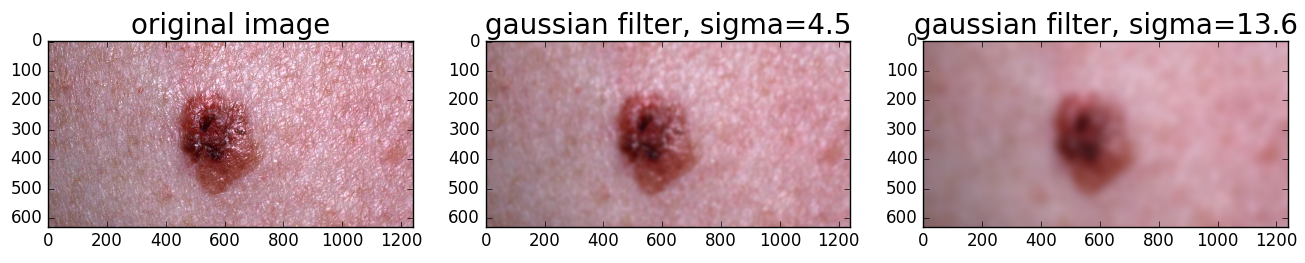
\includegraphics[width=\textwidth,keepaspectratio]{assets/image_processing/noise_reduction/gaussian/figure_01.png}
    \caption{Gaussian Filter Example A}
    \label{fig:med_A}
\end{figure}
\begin{figure}[H]
    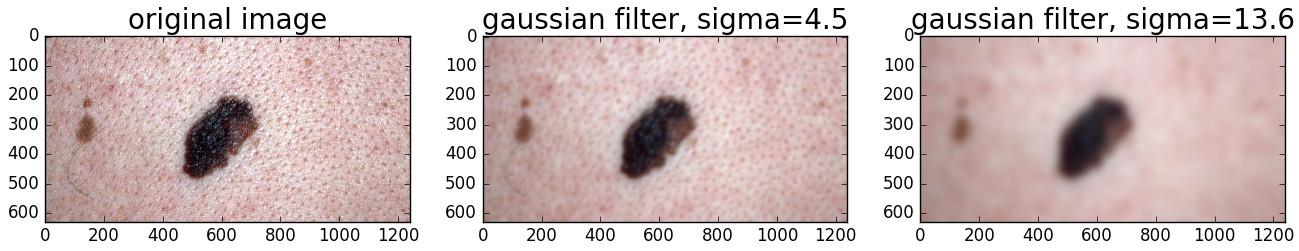
\includegraphics[width=\textwidth,keepaspectratio]{assets/image_processing/noise_reduction/gaussian/figure_02.png}
    \caption{Gaussian Filter Example B}
    \label{fig:med_B}
\end{figure}

In figure \ref{fig:med_B} there is a hair in the lower left side of the image. At higher sigma values the hair is still partially present, while the border of the lesion has already lost much detail. The tradeoff between noise reduction and loss of important detail is not optimal for the Gaussian filter.

\subsubsection{Median Filter}

The median filter will iterate through the pixels of an image, analysing each pixel and it's immediate neighbours. The value chosen for a pixels will be the median value of the area around the pixel. In a 2D context, if the neighbourhood around a pixel is [2,1,96] the pixel will receive the value 2. The median filter is easy to compute and has the quality that edges remain well preserved. This is therefore particularly useful as a preprocessing step before segmentation.

The following figures \ref{fig:med_A} to \ref{fig:med_C} are examples of median filtered images.

\begin{figure}[H]
    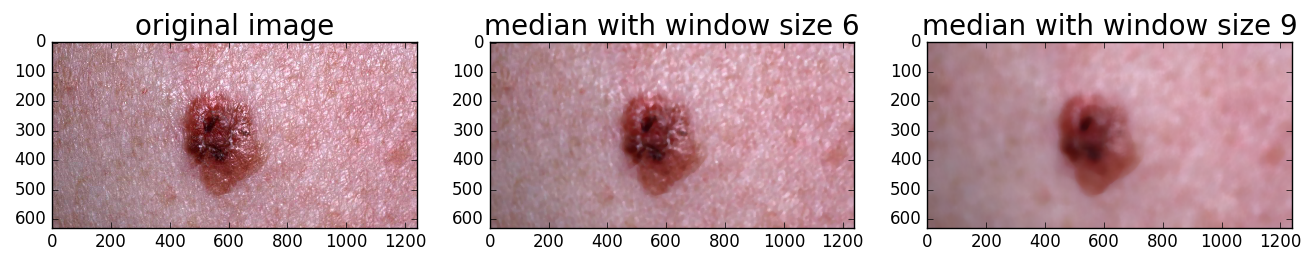
\includegraphics[width=\textwidth,keepaspectratio]{assets/image_processing/noise_reduction/figure_01.png}
    \caption{Median Filter Example A}
    \label{fig:med_A}
\end{figure}
\begin{figure}[H]
    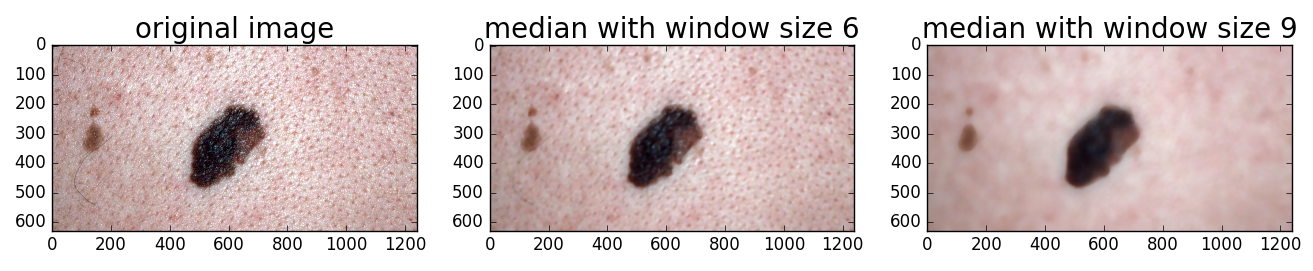
\includegraphics[width=\textwidth,keepaspectratio]{assets/image_processing/noise_reduction/figure_02.png}
    \caption{Median Filter Example B}
    \label{fig:med_B}
\end{figure}
\begin{figure}[H]
    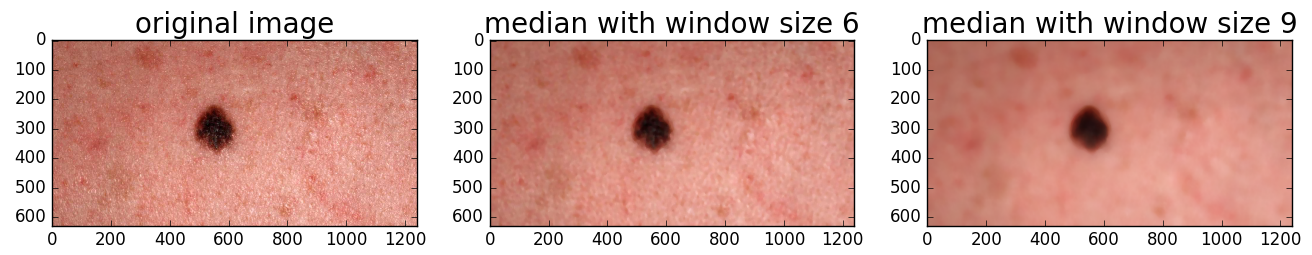
\includegraphics[width=\textwidth,keepaspectratio]{assets/image_processing/noise_reduction/figure_03.png}
    \caption{Median Filter Example C}
    \label{fig:med_B}
\end{figure}

The effect of the median window size is visible in the examples above. Larger window sizes are more effective at reducing noise and other disturbances. The edges of the lesion remain sharp, but the shape looses some detail, corners are rounded off. The size of the lesion in the image, and the image’s resolution are also important factors in the success of the median filter. If the lesion is too small compared to the image size, or the resolution of the image too low, then the shape will become more distorted. This will have a negative effect on the following segmentation steps.
\section{Segmentation}

\subsection{Iterative Thresholding}
\subsection{Region Selection}

\section{Image Feature Extraction}



\chapter{Machine Learning}
\section{Section Title}
\section{Results of Algorithm}

Performance Evaluation

Chapters from book 11.1, 11.2, 11.3, 11.5, 11.6

\chapter{Implementaion of the Algorithm}
\section{Section Title}

\chapter{Concept of the Application}
In section 2.2.1 categories of medical smart phone apps were defined. Apps in the same categories might have a similar feature set and capabilities. An app in the \textit{Alert / First Response} category might have a database that stores important contacts in the user’s area and a user interface that allows the user to quickly alert a contact in an emergency situation. An app in the \textit{Learning / Educational / Reference} category might be modelled as a quiz app which presents the user with a question and several possible answers to choose from. Answers from several questions will can be evaluated and a score is presented to the user at the end of a session. The app would be implemented with a database of questions and weighted answers, as well as an interface that presents the questions to the user sequentially.

One of the goals of this project is to define requirements for an app that provides a risk assessment of a lesion being benign or malignant. A high level description of the primary functionality of the app is the following:

\begin{itemize}[label={}]
\item The smart phone app allows the user to capture and analyse an image of a skin lesion and provide a risk assessment to the user of the lesion being a malignant melanoma.

\end{itemize}

The user might also like to save the image and results in oder to be able to compare it with other assessments in the future, or to review the assessment with a dermatologist. For comparison it might be useful to save associated metadata, such as the date and location on the body of the lesion. For convenience it might be nice to send the assessment and image via email to a specialist for review.
Secondary functionality can be described as follows:

\begin{itemize}[label={}]
\item The app allows the user to save or archive the image and corresponding assessment for future comparison and review.

\item The user can add, edit, and save metadata associated with the image of the lesion.
\item The user can browse archived images, assessments, and associated metadata.
\item The user can send a set of images with associated assessment and metadata via email.

\end{itemize}

From this high level description some basic assumptions about the app’s architecture can already be made. The app will require access to a database that can store information about an image, results of the analysis, and metadata. The app will require a user interface that allows a user to browse and edit data associated with an image. The app requires access to the smart phone’s camera api in order to capture images.

In order to formally elicit the requirements the hight level description will be broken down into structured use cases. A set of requirements will be extracted from the use cases.

\section{Use Cases}
In order to capture the formal use cases we will use a schema based on the one defined in Requirement Engineering Fundamentals \cite{9781937538774}.


\begin{table}[H]
    \begin{tabular}{ | >{\bfseries}l | p{8.35cm} |}
    \hline
    ID &  Unique designation of the use case \\ \hline
    Name & Unique name of the use case \\ \hline
    Priority & Importance of the use case according to applied prioritization technique \\ \hline
    Description &  Use case in user story form\\ \hline
    Dependencies & dependencies \\ \hline
    Trigger event & Name of the event that triggers this use case \\ \hline
    Actors & List of all the actors involved in this use case \\ \hline
    Preconditions & List of all necessary constraints that must be met before this use case can begin execution \\ \hline
    Posconditions & List of all states the system can be in immediately after the execution of the main scenario  \\ \hline
    Result & Description of the results that are produced during the use case execution \\ \hline
    Main scenario & Sequnce of events that occur during the use case. \\ \hline
    Alternate scenarios & Alternative sequence of events that might occur. \\ \hline

    Comments & Other infos \\ \hline
    \end{tabular}

    \caption{Use Case Template}
    \label{fig:uc_template}
\end{table}

\begin{table}[H]
    \begin{tabular}{ | >{\bfseries}l | p{9.5cm} |}
    \hline
    ID
    &  UC-1 \\ \hline
    Name
    & Capture Image \\ \hline
    Description
    &  As a user I can capture an image of the skin lesion that I would like to have analysed. \\ \hline
    Dependencies
    & None \\ \hline
    Trigger
    & The user activated the application and selected the "image capture" navigation item. \\ \hline
    Preconditions
    & The system state which must be active before the Use Case can occur \\ \hline
    Normal Flow
    &

    \begin{description}[align=left]
    \item [1.]Point the camera at the skin lesion.
    \item [2.]Rotate and move the camera until the skin lesion is centered and optimally sized.
    \item [3.]The user touches the screen to capture the image.
    \item [4.]The user is notified ( beep ) that the image has been captured
    \item [5.]The user can repeat from the begining
    \end{description}

    \\ \hline
    Alternate Flow & None \\ \hline
    Results
    & The captured images are placed by the system in a processing queue to calculate the lesion's border. \\ \hline
    Comments
    & It is important that a user can capture the image with just one hand. If a lesion is located on a user's hand or arm, it's not possible to use two hands. \\ \hline
    \end{tabular}

    \caption{Use Case 1}
    \label{fig:uc_1}
\end{table}
\begin{table}[H]
    \begin{tabular}{ | >{\bfseries}l | p{9.5cm} |}
    \hline
    ID
    &  UC-2 \\ \hline
    Name
    & Confirm correct calculation of skin lesion's border \\ \hline
    Description
    &  As a user I want to confirm that the skin lesion's borders have been properly calculated. \\ \hline
    Dependencies
    & UC-1 \\ \hline
    Trigger
    & The user selected the "confirm border" navigation item. \\ \hline
    Preconditions
    & At least one image has been queued for border calculation. \\ \hline
    Normal Flow
    &
    \begin{description}[align=left]
    \item [1.]The user is presented with a list of images.
    \item [2.]The following step is repeated for each image in the list.
    \item [3.]The user confirms that the border of the lesion has been precisely calculated.
    \end{description}
    \\ \hline
    Alternate Flow
    &
    \begin{description}[align=left]
    \item [A1.] Border calculation for image has not completed.
    \item [A1.3] The user can refresh the image preview until the results of the border are visible.
    \item [A1.4] The user confirms that the border of the lesion has been precisely calculated.
    \end{description}
    \begin{description}[align=left]
    \item [A2] Border calculation is not precise or has failed.
    \item [A2.3] The user confirms that the border of the lesion has not been precisely calculated.
    \item [A2.4] The image is deleted.
    \end{description}
    \\ \hline
    Results
    & After positiv confirmation, images are placed by the system in the risk assessment calculation queue.
If no images can be positively confirmed, the user can recapture new images ( UC-1 ) \\ \hline
    Comments
    & It is important that a user can capture the image with just one hand. If a lesion is located on a user's hand or arm, it's not possible to use two hands. \\ \hline
    \end{tabular}

    \caption{Use Case 2}
    \label{fig:uc_2}
\end{table}
\begin{table}[H]
    \begin{tabular}{ | >{\bfseries}l | p{9.5cm} |}
    \hline
    ID
    &  UC-3 \\ \hline
    Name
    & View risk assessment \\ \hline
    Description
    &  As a user I want to view the results of the risk assessment calculation. \\ \hline
    Dependencies
    & UC-2 \\ \hline
    Trigger
    & The user selected the "risk assessment results" navigation item. \\ \hline
    Preconditions
    & The system was able to complete the risk assessment calculation \\ \hline
    Normal Flow
    &
    \begin{description}[align=left]
    \item [1.]The user is presented with a list of images.
    \item [2.]The following step is repeated for each image in the list.
    \item [3.]The user can select and view and image and corresponding results in detail.
    \end{description}
    \\ \hline
    Alternate Flow
    &
    \begin{description}[align=left]
    \item [A1.] Risk assessment calculation for image has not completed.
    \item [A1.3] The user can refresh the results details until the results of a risk assessment is available.
    \end{description}

    \\ \hline
    Results
    &  \\ \hline
    Comments
    &  \\ \hline
    \end{tabular}

    \caption{Use Case 3}
    \label{fig:uc_3}
\end{table}
\section{Section Title}
\begin{table}[H]
    \begin{tabular}{ | >{\bfseries}l | p{9.5cm} |}
    \hline
    ID
    &  UC-5 \\ \hline
    Name
    & View archived images and data. \\ \hline
    Description
    &  As a user I want to view previously saved images and the corresponding risk assessment data. \\ \hline
    Dependencies
    & UC-4 \\ \hline
    Trigger
    & The user selects the "archive" navigation item. \\ \hline
    Preconditions
    & The system was able to complete the risk assessment calculation. \\ \hline
    Normal Flow
    &
    \begin{description}[align=left]
    \item [1.]The user is presented with a list of archived packages.
    \item [2.]The user can select an item in the list
    \item [3.]The user is presented with the images, corresponding risk assessment data and metadata for the selected item.
    \end{description}
    \\ \hline
    Alternate Flow
    &

    \\ \hline
    Results
    &
    A package of images and corresponding risk assessment data is stored in the archive with some metadata (title and comment).
    \\ \hline
    Comments
    &  \\ \hline
    \end{tabular}

    \caption{Use Case 5}
    \label{fig:uc_5}
\end{table}
\begin{table}[H]
    \begin{tabular}{ | >{\bfseries}l | p{9.5cm} |}
    \hline
    ID
    &  UC-6 \\ \hline
    Name
    & Send results to dermatologist. \\ \hline
    Description
    &  As a user I want to send a previously saved image, feature extraction data and assessment results to a dermatologist. \\ \hline
    Dependencies
    & UC-4 \\ \hline
    Trigger
    & The user selects the "archive" navigation item. \\ \hline
    Preconditions
    & The system was able to complete the risk assessment calculation. \\ \hline
    Normal Flow
    &
    \begin{description}[align=left]
    \item [1.]The user is presented with a list of archived packages.
    \item [2.]The user can select an item in the list
    \item [3.]The user can send the item as an email attachment.
    \end{description}
    \\ \hline
    Alternate Flow
    &

    \\ \hline
    Results
    &
    \\ \hline
    Comments
    &  \\ \hline
    \end{tabular}

    \caption{Use Case 6}
    \label{fig:uc_6}
\end{table}



\section{User Interface}
\begin{figure}[H]
\centering
    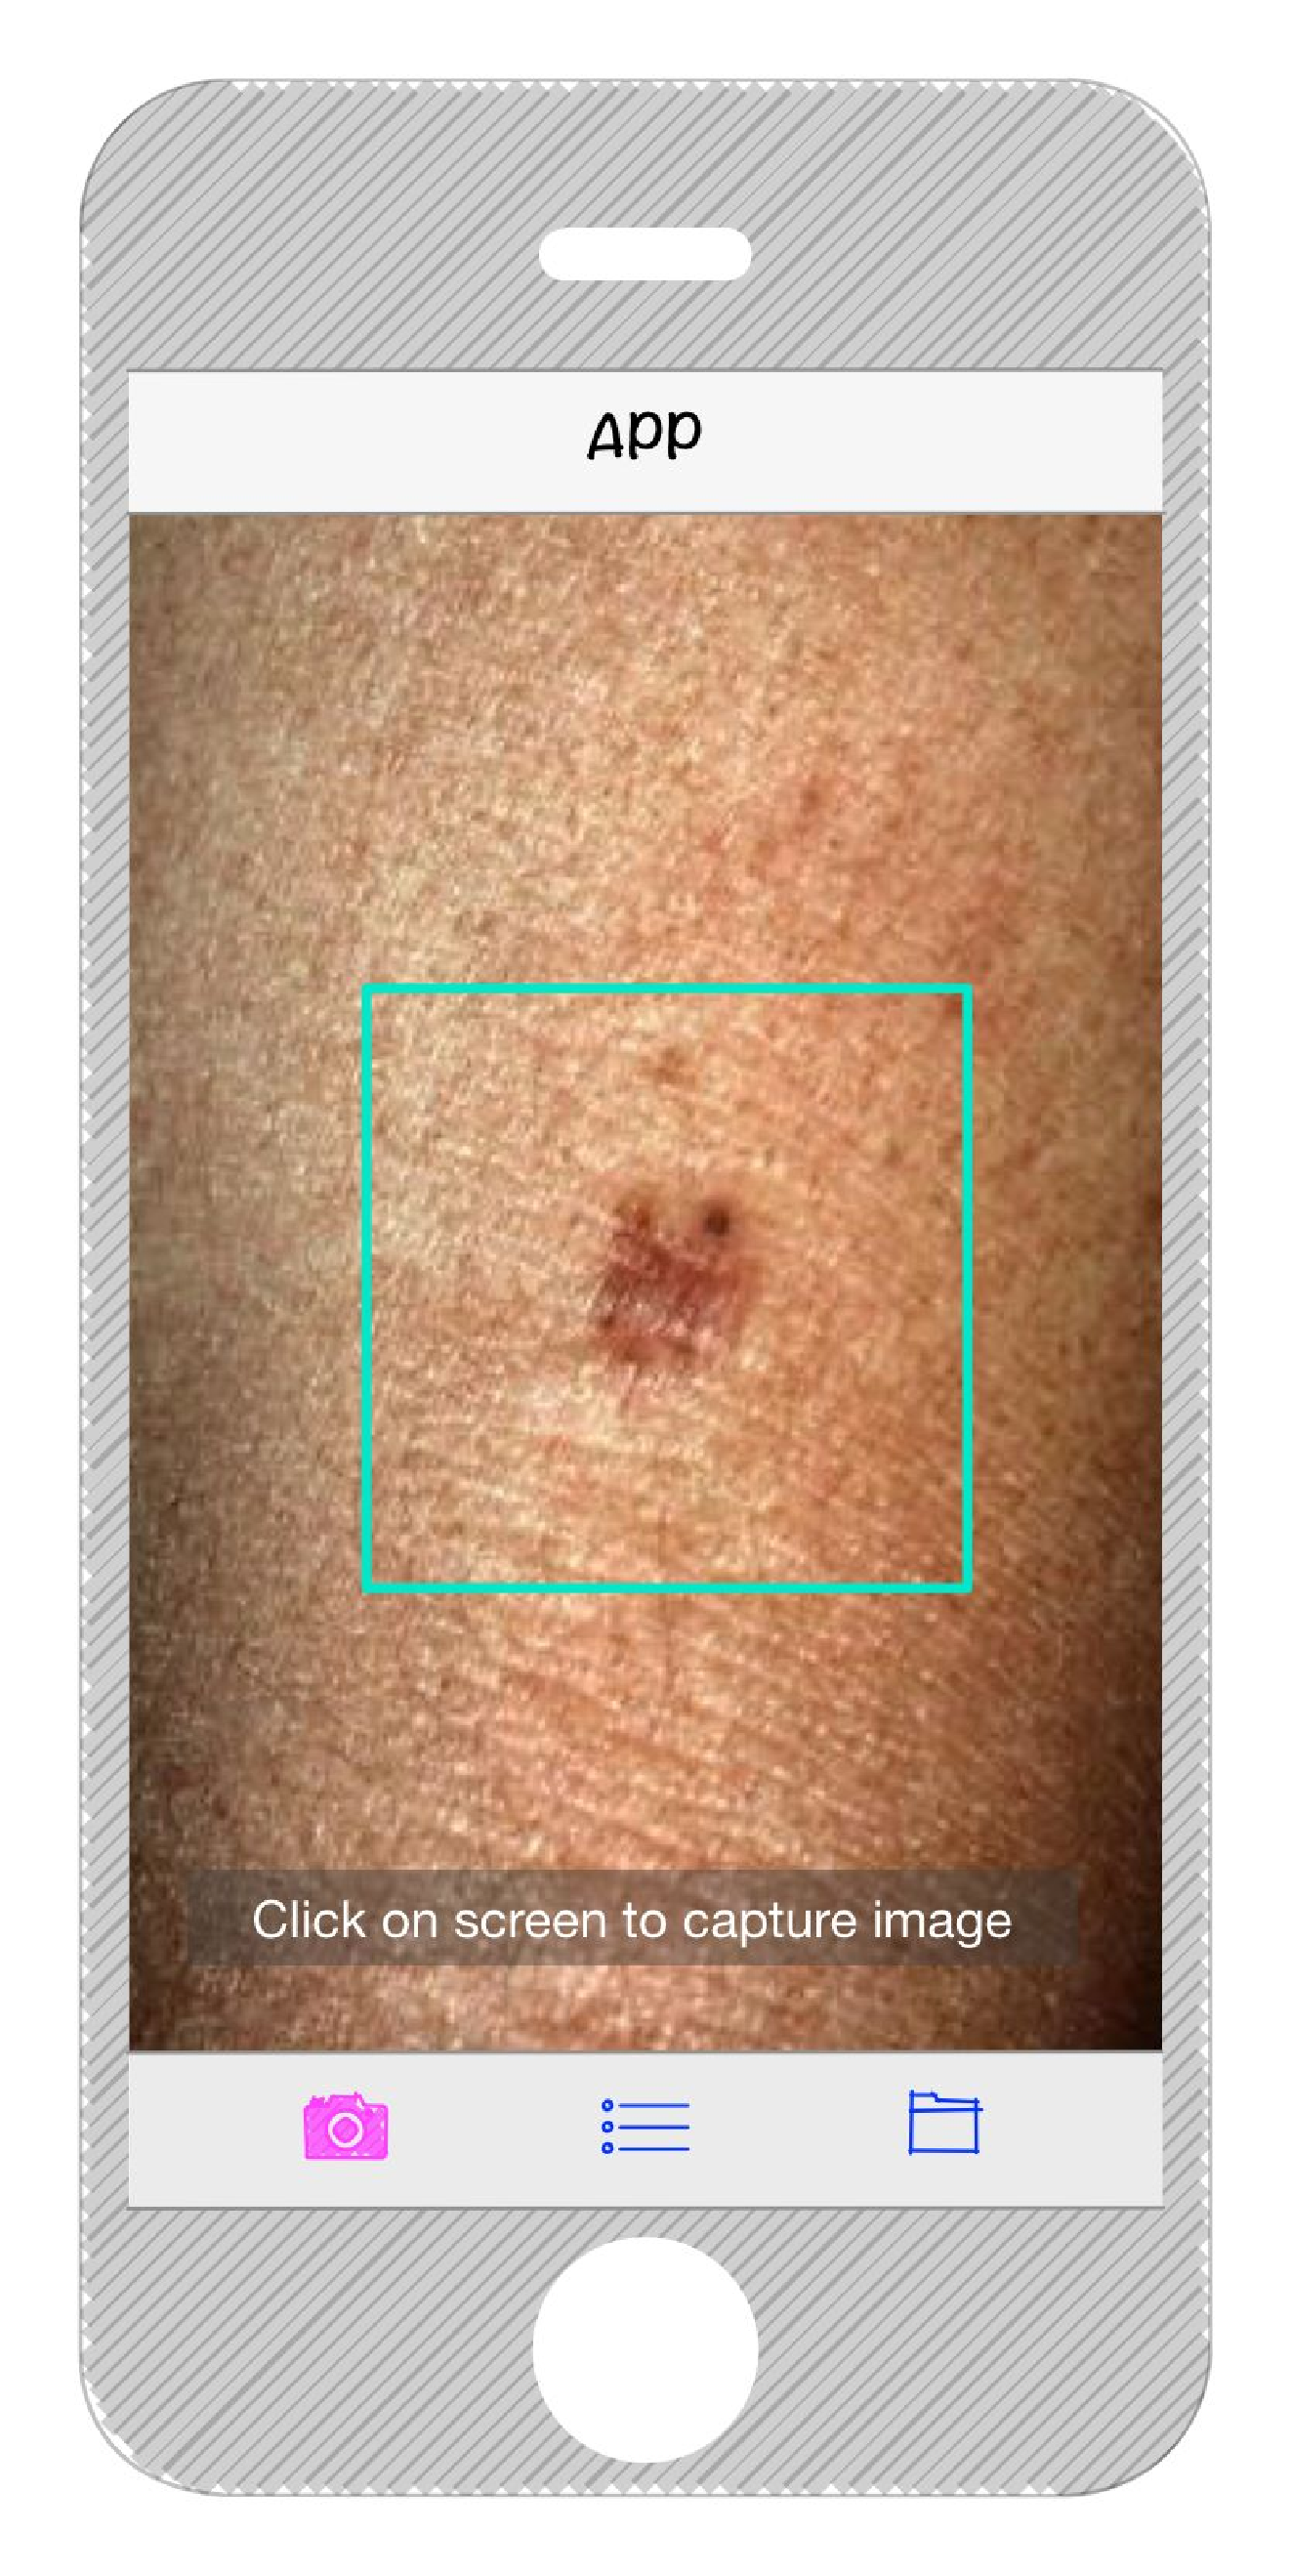
\includegraphics[height=10cm,keepaspectratio]{assets/GUI/image_capture.pdf}
    \caption{Image Capture View}
    \label{fig:image_capture}
\end{figure}

\begin{figure}[H]
    \centering
    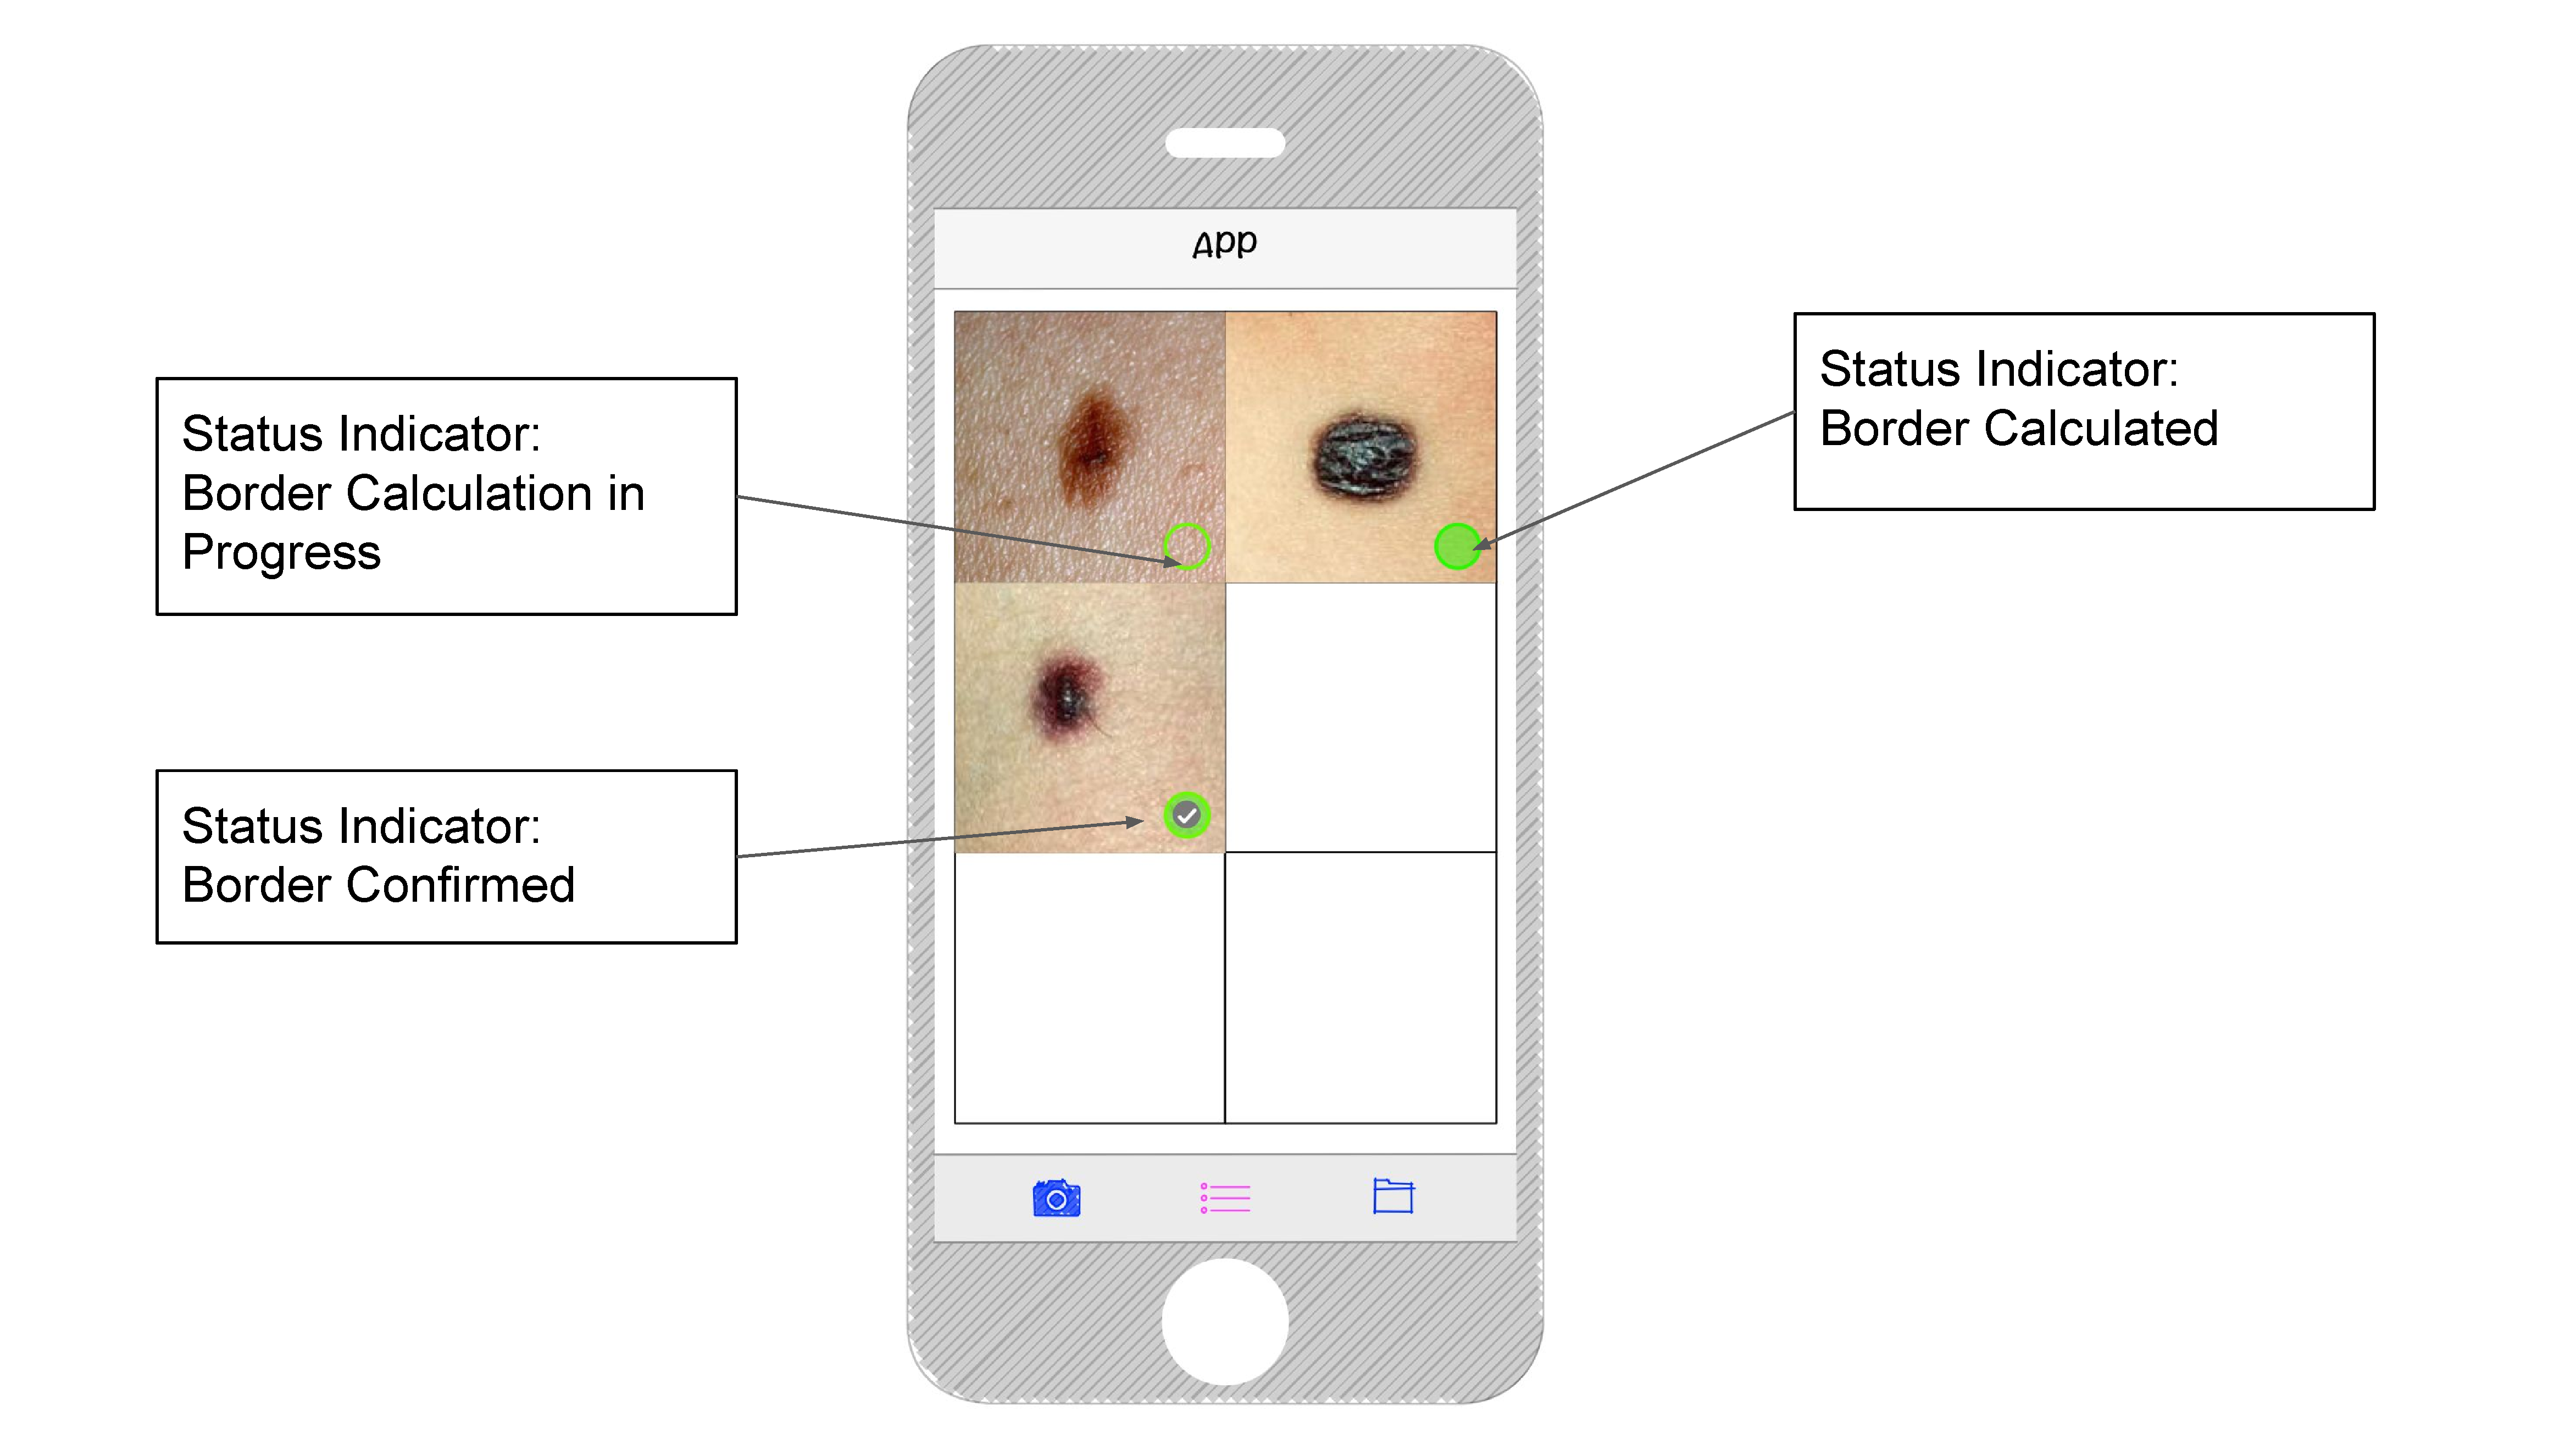
\includegraphics[height=10cm,keepaspectratio]{assets/GUI/image_list_view.pdf}
    \caption{Image List View}
    \label{fig:image_list_view}
\end{figure}

\begin{figure}[H]
    \centering
    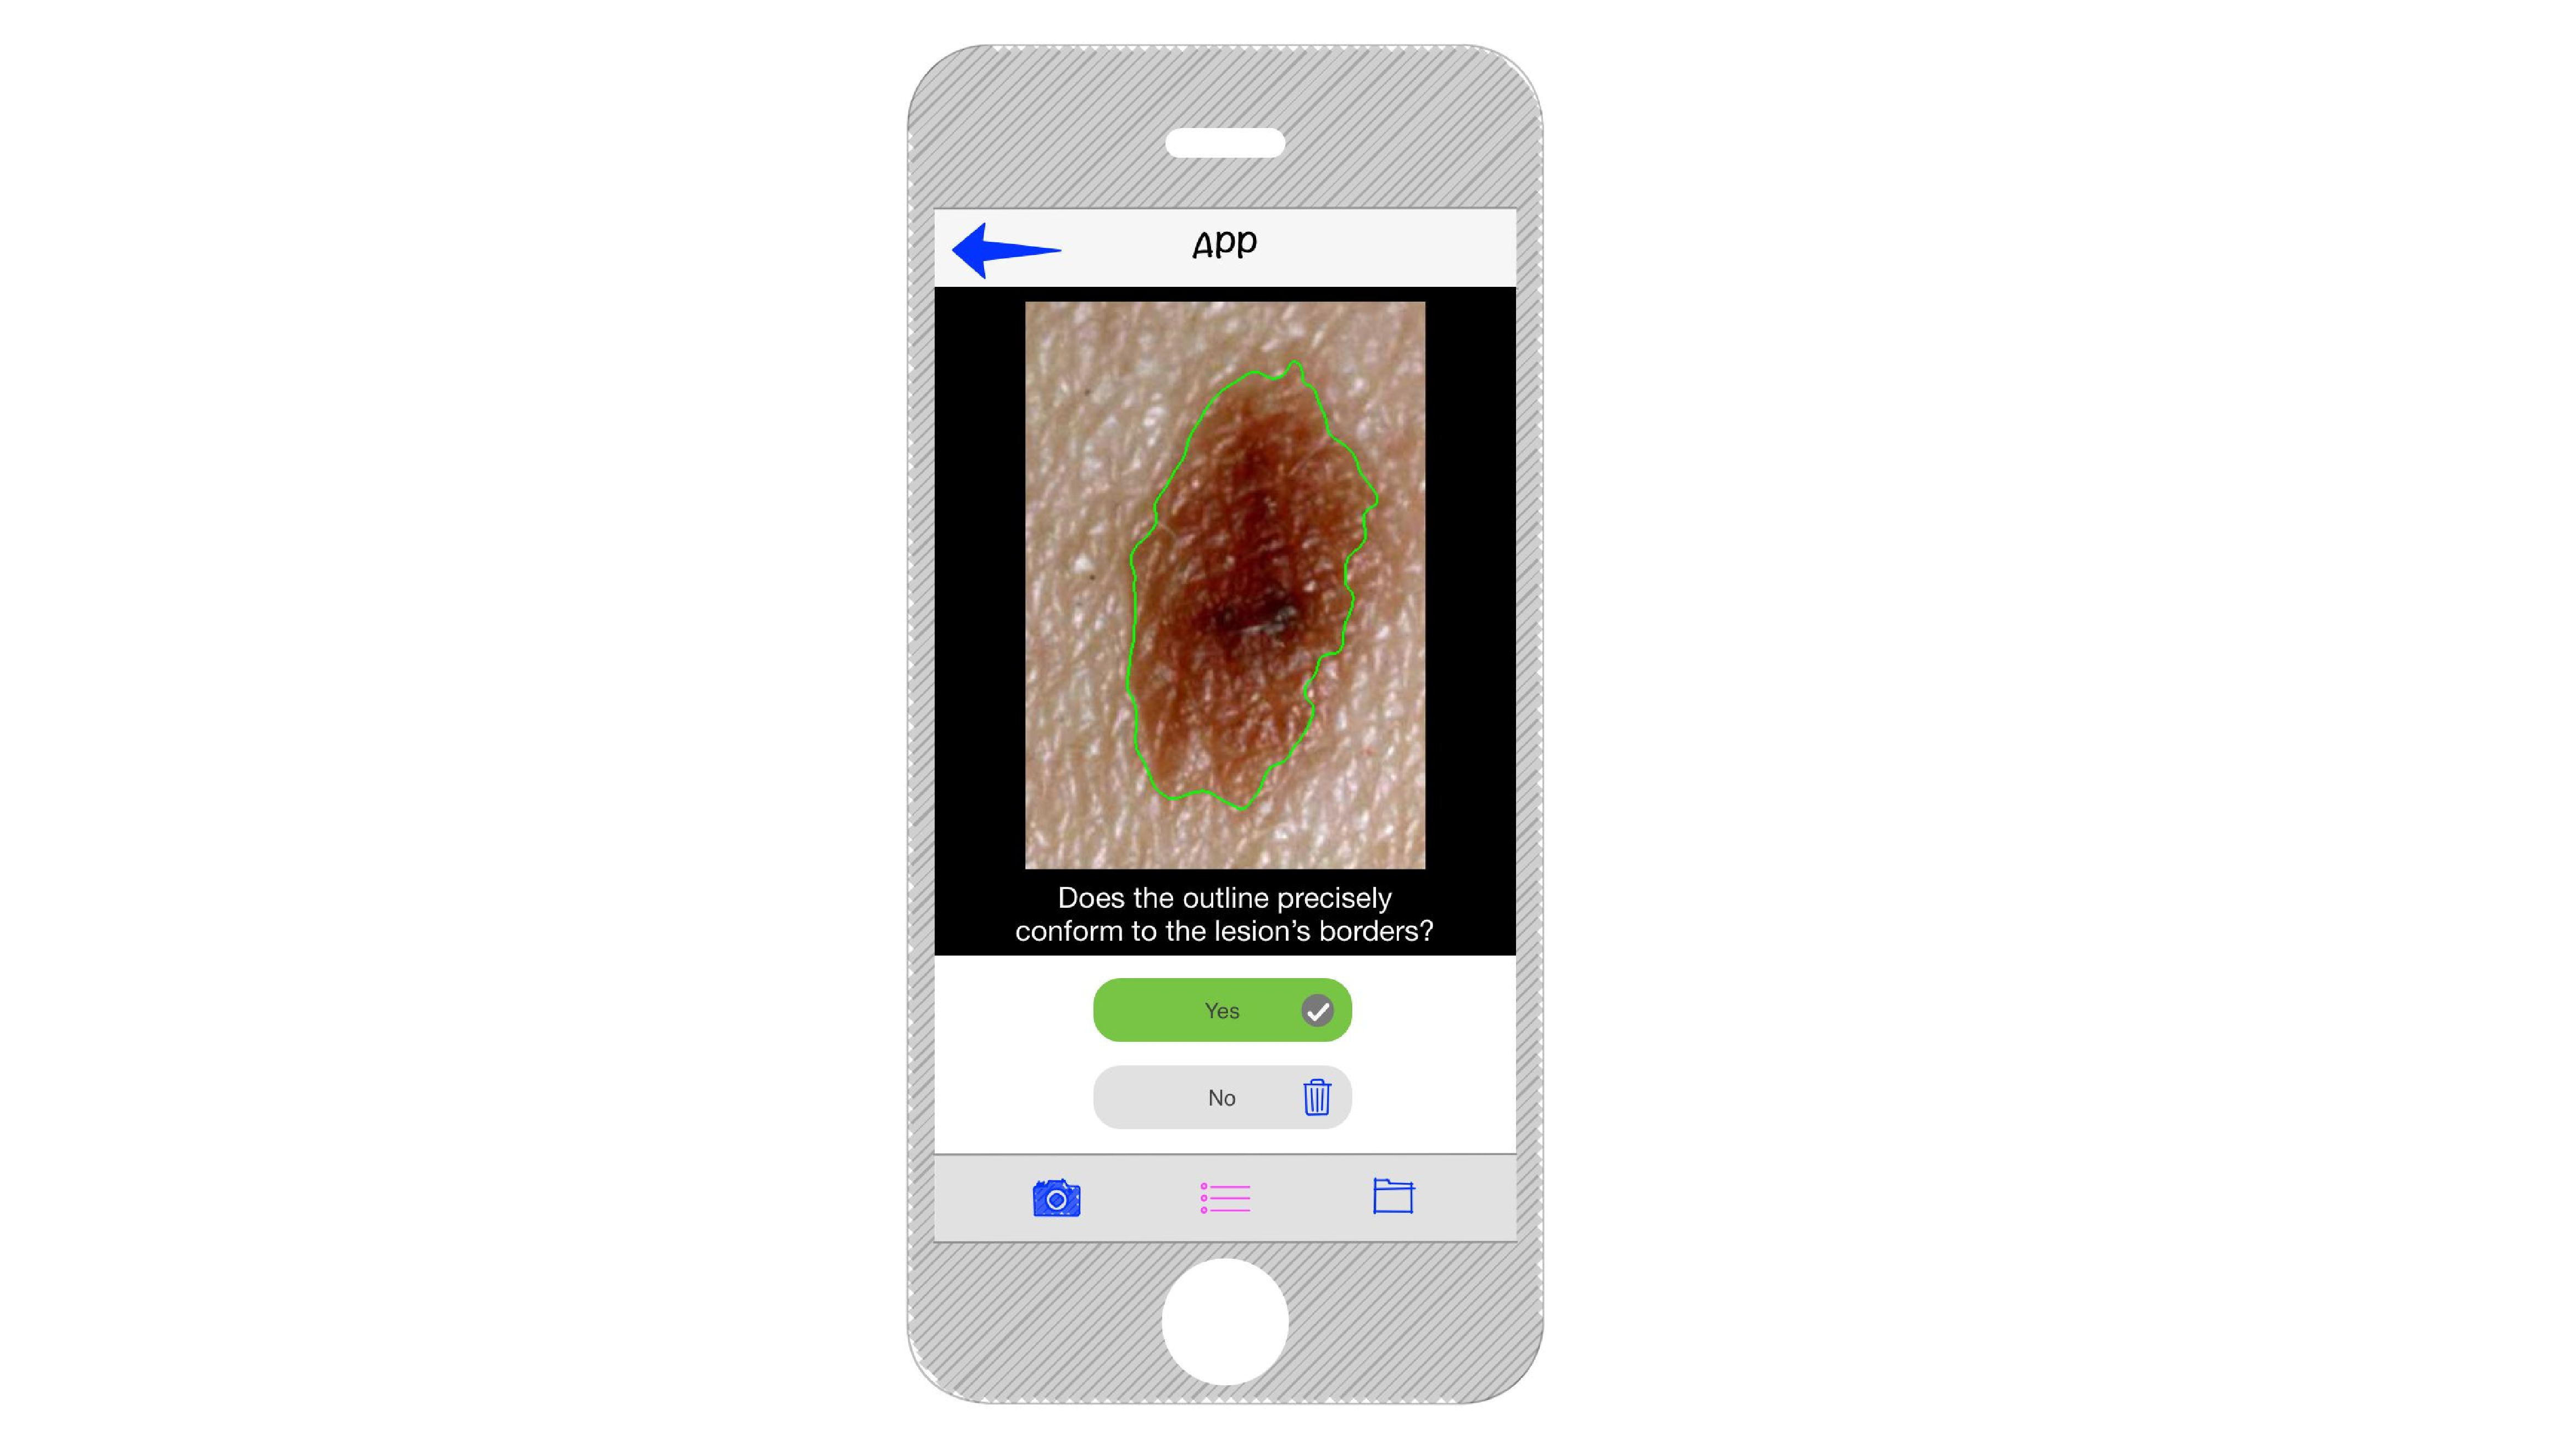
\includegraphics[height=10cm,keepaspectratio]{assets/GUI/border_confirm.pdf}
    \caption{Border Confirm View}
    \label{fig:border_confirm_view}
\end{figure}

\begin{figure}[H]
    \centering
    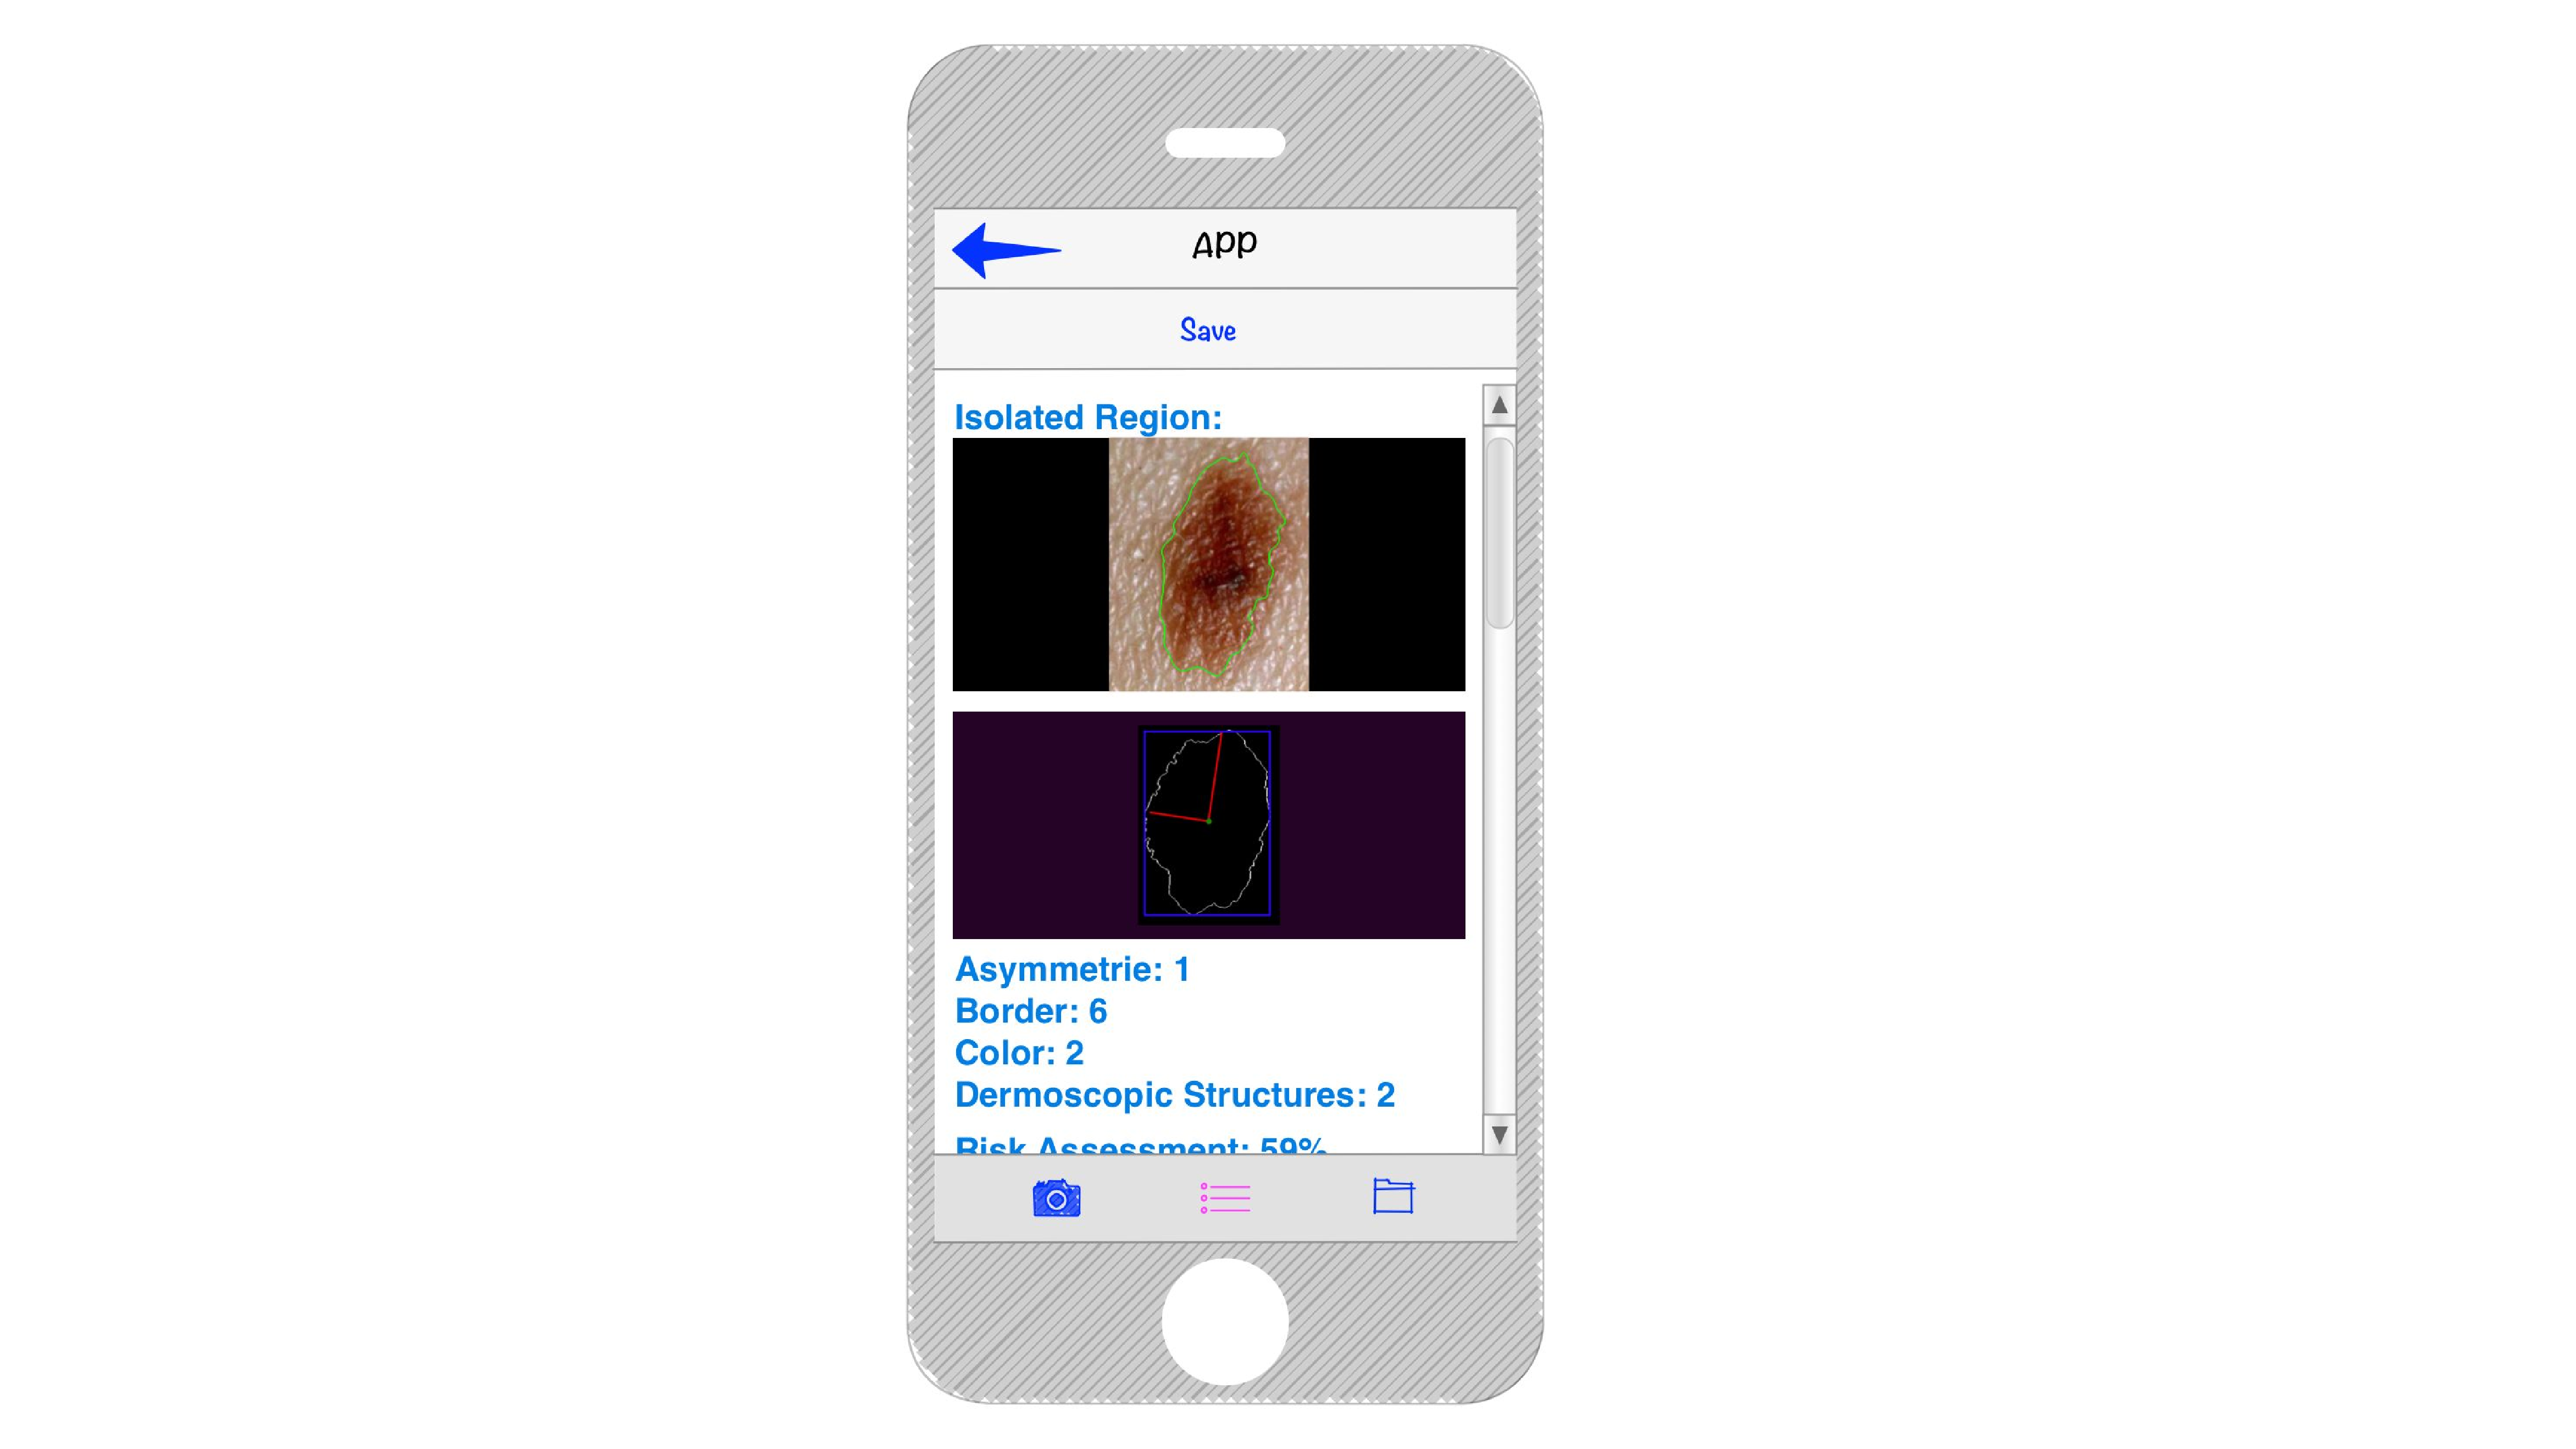
\includegraphics[height=10cm,keepaspectratio]{assets/GUI/image_detail_view.pdf}
    \caption{Image Detail View}
    \label{fig:image_detail_view}
\end{figure}

\begin{figure}[H]
    \centering
    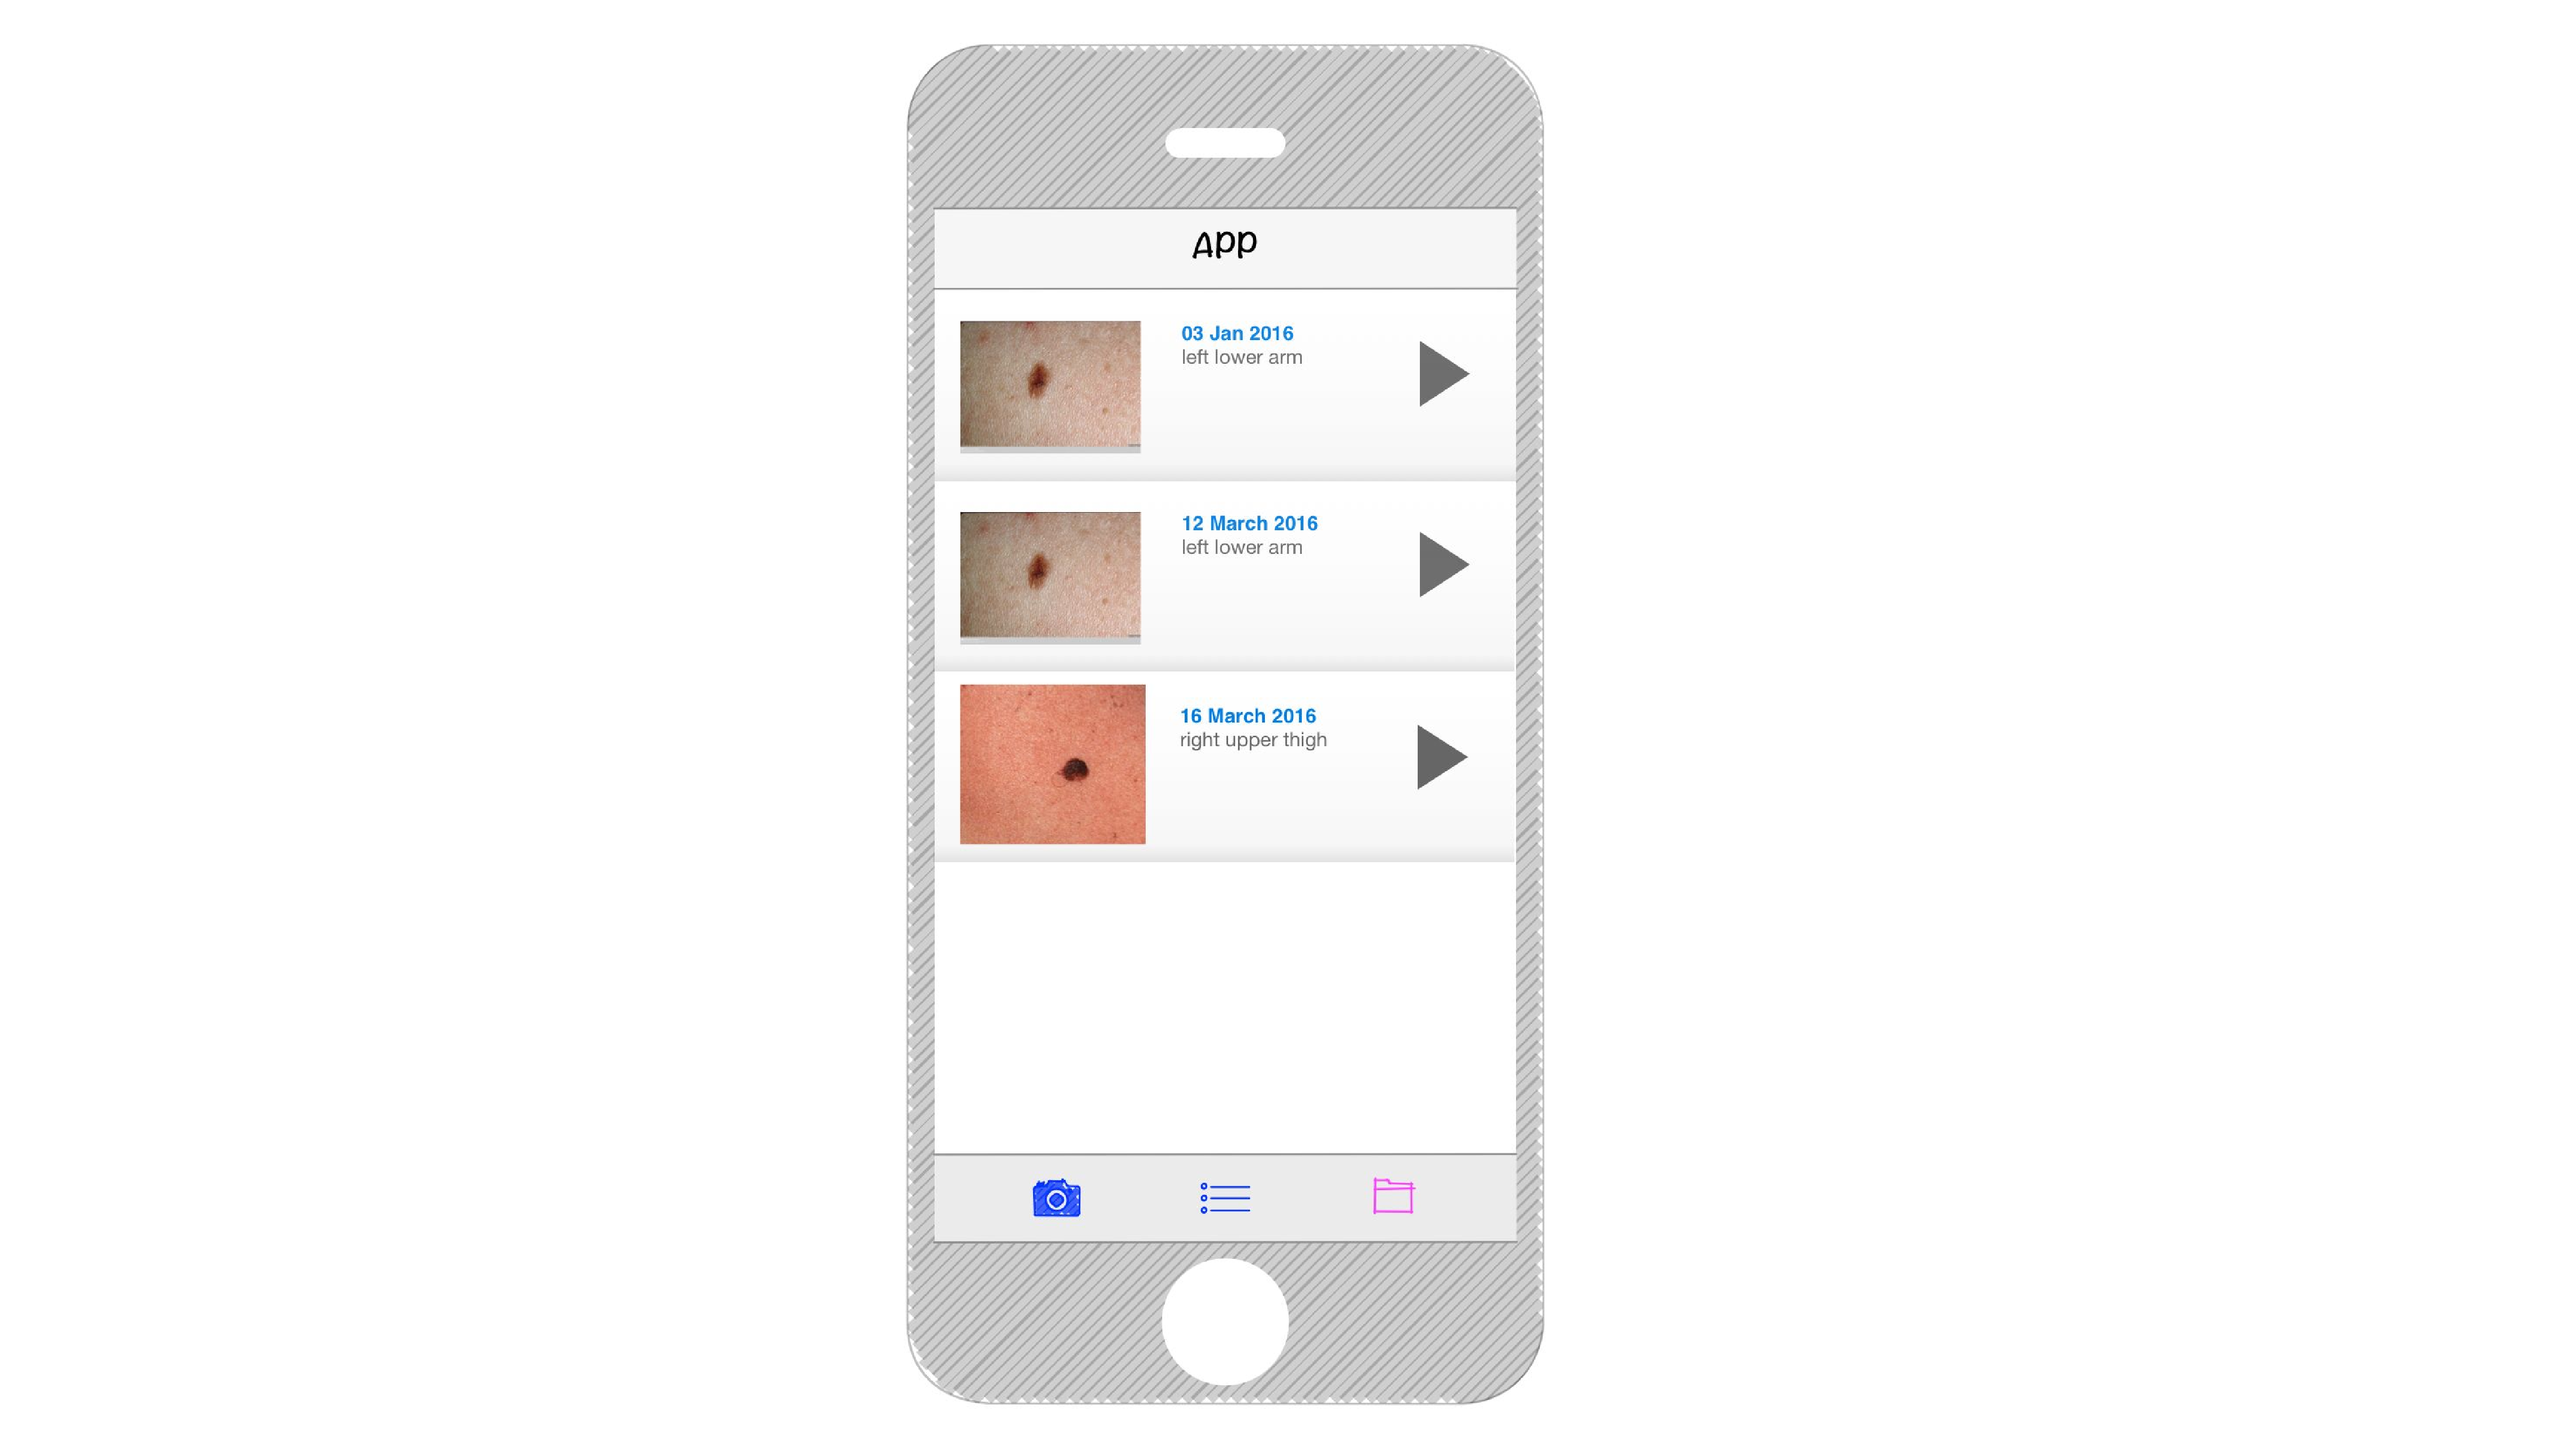
\includegraphics[height=10cm,keepaspectratio]{assets/GUI/archive_view.pdf}
    \caption{Archive View}
    \label{fig:archive_view}
\end{figure}

\begin{figure}[H]
    \centering
    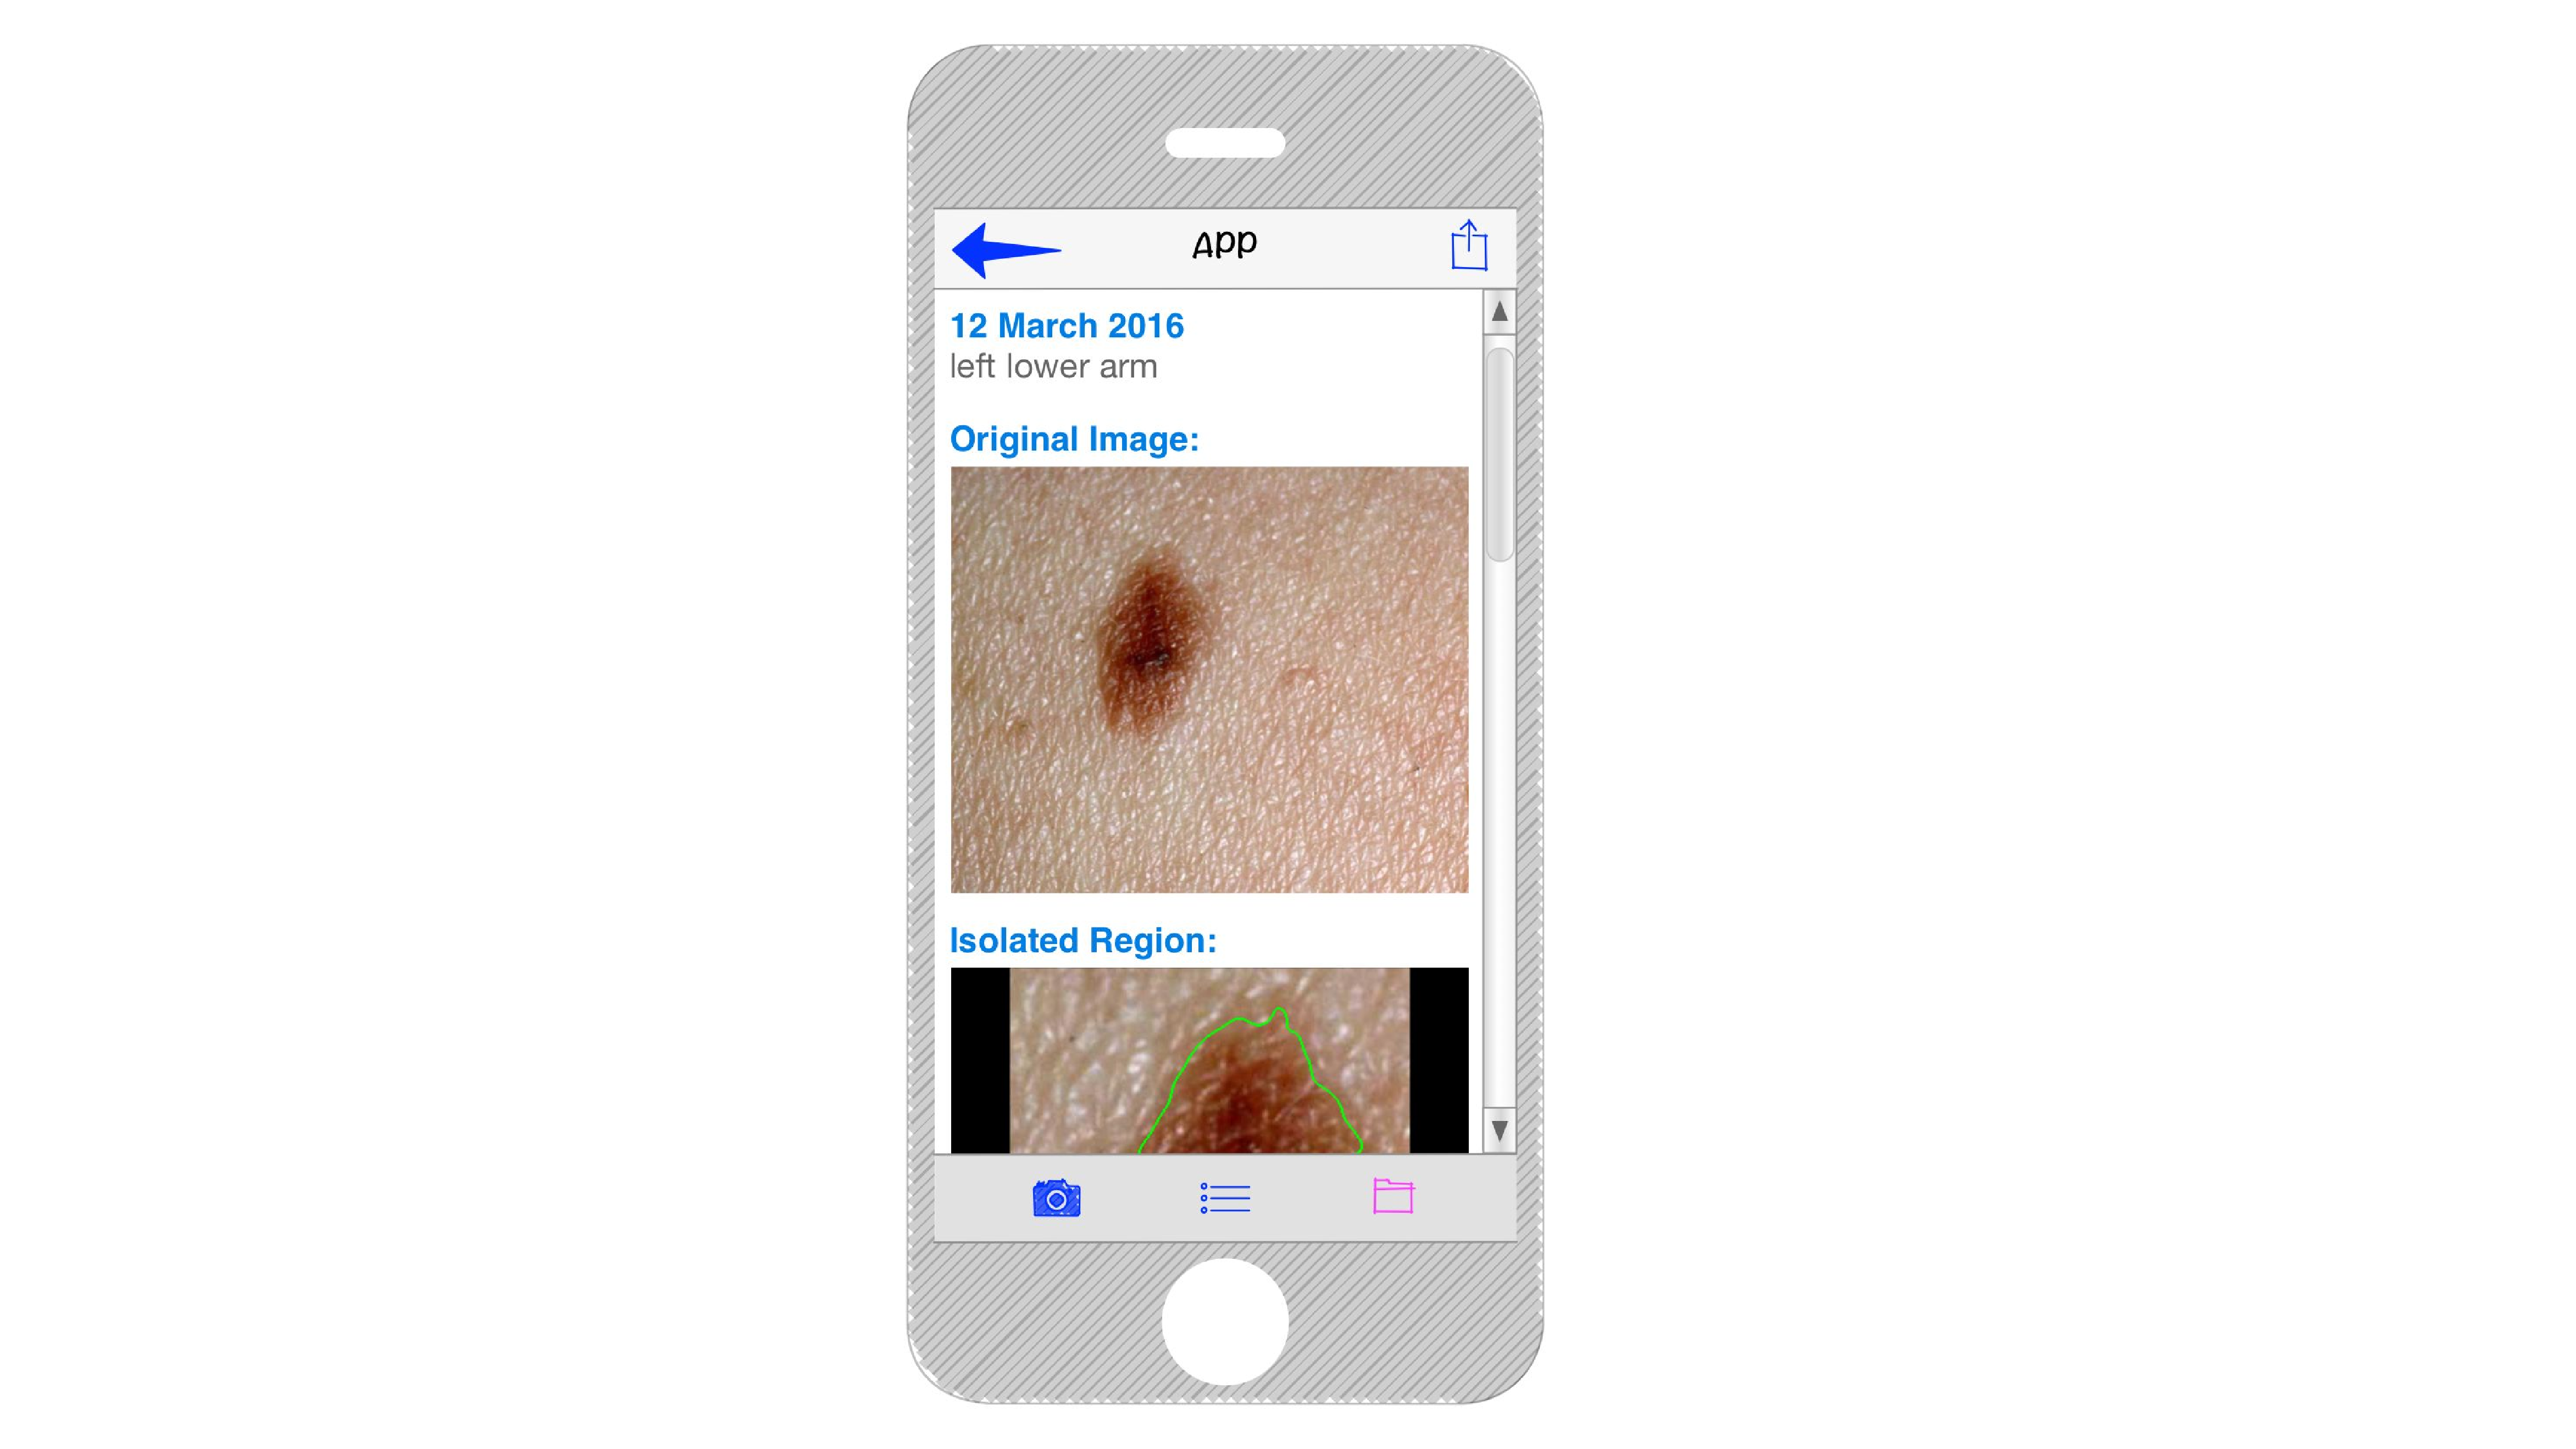
\includegraphics[height=10cm,keepaspectratio]{assets/GUI/archive_detail_view.pdf}
    \caption{Archive Detail View}
    \label{fig:archive_detail}
\end{figure}

\section{Requirements}

\section{Prioritized Requirements}

\begin{longtable}{ | l | l | l | l | l | l | l |}
\hline
ID & Priority & Name & Implemented  \\ \hline

REQ-F-1 & - & Preview Camera Input & -  \\ \hline
REQ-F-2 & - & Capture Camera Input & -  \\ \hline
REQ-F-3 & - & Border Extraction & -  \\ \hline
REQ-F-4 & - & Browse Images and Results & -  \\ \hline
REQ-F-5 & - & Select Image To View in Detail & -  \\ \hline
REQ-F-6 & - & Border Confirmation & -  \\ \hline
REQ-F-7 & - & Feature Extraction & -  \\ \hline
REQ-F-8 & - & Feature Extraction & -  \\ \hline


\caption{Prioritzed Requirement List}
\label{fig:prio_req}
\end{longtable}

\begin{table}[H]
    \begin{tabular}[t]{ | >{\bfseries}l | p{9.5cm} |}

    \hline
    ID
    &  REQ-F-1 \\ \hline

    Name
    & Preview Camera Input \\ \hline

    Description
    &  The system will let the user view a preview of the camera's input in realtime \\ \hline

    Preconditions
    & None \\ \hline

    Acceptance Tests
    & \\ \hline

    Relations
    & UC-1 \\ \hline

    Comments
    &  \\ \hline

    \end{tabular}

    \caption{Functional Requirement 1}
    \label{fig:req_f_1}

\end{table}
\begin{table}[H]
    \begin{tabular}[t]{ | >{\bfseries}l | p{9.5cm} |}

    \hline
    ID
    &  REQ-F-2 \\ \hline

    Name
    & Capture Camera Input \\ \hline

    Description
    &  The system will let the user capture an image from the camera's input. \\ \hline

    Preconditions
    & None \\ \hline

    Acceptance Tests
    & \\ \hline

    Relations
    & UC-1 \\ \hline

    Comments
    &  \\ \hline

    \end{tabular}

    \caption{Functional Requirement 2}
    \label{fig:req_f_2}

\end{table}
\begin{table}[H]
    \begin{tabular}[t]{ | >{\bfseries}l | p{9.5cm} |}

    \hline
    ID
    &  REQ-F-3 \\ \hline

    Name
    & Border Extraction \\ \hline

    Description
    &  The system must be able to calculate the border of a lesion in a captured image. \\ \hline

    Preconditions
    & None \\ \hline

    Acceptance Tests
    & \\ \hline

    Relations
    & UC-2 \\ \hline

    Comments
    &  \\ \hline

    \end{tabular}

    \caption{Functional Requirement 3}
    \label{fig:req_f_3}

\end{table}
\begin{table}[H]
    \begin{tabular}[t]{ | >{\bfseries}l | p{9.5cm} |}

    \hline
    ID
    &  REQ-F-4 \\ \hline

    Name
    & Browse Images and Results \\ \hline

    Description
    &  The system will let the user browse through a list of images. The list will display the status of the images. \\ \hline

    Preconditions
    & None \\ \hline

    Acceptance Tests
    & \\ \hline

    Relations
    &  \\ \hline

    Comments
    &  \\ \hline

    \end{tabular}

    \caption{Functional Requirement 4}
    \label{fig:req_f_4}

\end{table}
\begin{table}[H]
    \begin{tabular}[t]{ | >{\bfseries}l | p{9.5cm} |}

    \hline
    ID
    &  REQ-F-5 \\ \hline

    Name
    & Select Image To View in Detail \\ \hline

    Description
    &  The system will let the user select and view an image as well as the results of completed processes. \\ \hline

    Preconditions
    & None \\ \hline

    Acceptance Tests
    & \\ \hline

    Relations
    &  \\ \hline

    Comments
    &  \\ \hline

    \end{tabular}

    \caption{Functional Requirement 5}
    \label{fig:req_f_5}

\end{table}
\begin{table}[H]
    \begin{tabular}[t]{ | >{\bfseries}l | p{9.5cm} |}

    \hline
    ID
    &  REQ-F-6 \\ \hline

    Name
    & Border Confirmation \\ \hline

    Description
    & The system will let the user confirm that the border of a lesion hat been precisely calculated. \\ \hline

    Preconditions
    &  \\ \hline

    Acceptance Tests
    & \\ \hline

    Relations
    &  \\ \hline

    Comments
    &  \\ \hline

    \end{tabular}

    \caption{Functional Requirement 6}
    \label{fig:req_f_6}

\end{table}
\begin{table}[H]
    \begin{tabular}[t]{ | >{\bfseries}l | p{9.5cm} |}

    \hline
    ID
    &  REQ-F-7 \\ \hline

    Name
    & Feature Extraction \\ \hline

    Description
    & The system must be able to extract relavent features from the isolated lesion image. \\ \hline

    Preconditions
    &  \\ \hline

    Acceptance Tests
    & \\ \hline

    Relations
    &  \\ \hline

    Comments
    &  \\ \hline

    \end{tabular}

    \caption{Functional Requirement 7}
    \label{fig:req_f_7}

\end{table}
\begin{table}[H]
    \begin{tabular}[t]{ | >{\bfseries}l | p{9.5cm} |}

    \hline
    ID
    &  REQ-F-8 \\ \hline

    Name
    & Add To Process Queue \\ \hline

    Description
    & The system must be able to add an image process job to the process queue \\ \hline

    Preconditions
    &  \\ \hline

    Acceptance Tests
    & \\ \hline

    Relations
    &  \\ \hline

    Comments
    &  \\ \hline

    \end{tabular}

    \caption{Functional Requirement 8}
    \label{fig:req_f_8}

\end{table}
\begin{table}[H]
    \begin{tabular}[t]{ | >{\bfseries}l | p{9.5cm} |}

    \hline
    ID
    &  REQ-F-9 \\ \hline

    Name
    & Add/Save/Edit Metadata to Image and Results \\ \hline

    Description
    & The system will allow the user to add or edit metadata associated with the captured image. \\ \hline

    Preconditions
    &  \\ \hline

    Acceptance Tests
    & \\ \hline

    Relations
    &  \\ \hline

    Comments &
        The metadata associated might include the date when the image was captures as well as the location on the body where the lesion is located. The metadata will have the form of a text input field where the user can enter any text. It could be extended, if necessary, with structured data fields.

    \\ \hline

    \end{tabular}

    \caption{Functional Requirement 9}
    \label{fig:req_f_9}

\end{table}
\begin{table}[H]
    \begin{tabular}[t]{ | >{\bfseries}l | p{9.5cm} |}

    \hline
    ID
    &  REQ-F-10 \\ \hline

    Name
    & Save Image and Associated Data as Archive. \\ \hline

    Description
    & The system will allow the user to save images and associated data for reassessment and comparison in the future. \\ \hline

    Preconditions
    &  \\ \hline

    Acceptance Tests
    & \\ \hline

    Relations
    &  \\ \hline

    Comments &

        Storage on a mobile device is a limited resource. Depending on the development strategy chosen, Web App vs Native, the application might not have access to it's own data store. It would be useful to offload data to a cloud or web based storage location.

    \\ \hline

    \end{tabular}

    \caption{Functional Requirement 10}
    \label{fig:req_f_10}

\end{table}
\begin{table}[H]
    \begin{tabular}[t]{ | >{\bfseries}l | p{9.5cm} |}

    \hline
    ID
    &  REQ-F-11 \\ \hline

    Name
    & Browse Images and Results from Archive. \\ \hline

    Description
    & The sytem will allow the user to browse previously saved images and results from the archive. \\ \hline

    Preconditions
    &  \\ \hline

    Acceptance Tests
    & \\ \hline

    Relations
    &  \\ \hline

    Comments
    &  \\ \hline

    \end{tabular}

    \caption{Functional Requirement 11}
    \label{fig:req_f_11}

\end{table}

\section{Prioritisation}
This project will employ a Single-Criterion Ad-hoc prioritisation classification as opposed to an analytical approach such as the Wiegers prioritisation matrix. The rationale behind this choice is that as a single person development project the determination of weights for benefit, detriment, cost, and risk is an ad-hoc exercise. In a larger project with multiple developers and active stakeholders the time and effort required for a prioritisation assessment according to Wiegers would be advisable.

The following are the prioritisation classes as defined in \cite{9781937538774}:

\begin{itemize}[label={}]

\item \textbf{Mandatory}: A mandatory requirement is a requirement that must be implemented at all costs or else the success of the system is threatened.
\item \textbf{Optional}: An optional requirement is a requirement that does not necessarily need to be implemented. Neglecting a few requirements of this class does not threaten the success of the system.
\item \textbf{Nice-to-have}: Nice-to-have requirements are requirements that do not influence the system’s success if they are not implemented.

\end{itemize}



\section{Software Architecture}
\subsection{MVC}
Since the 1970s the Model View Controller ( MVC ) pattern is the standard architectural design pattern for applications that present the user with a graphical user interface. It was developed out of a need for modularity, to encapsulate responsibility of specific concepts to separate program modules, or Separation of Concerns. MVC identifies three main components that program code should be grouped into, namely\cite{walther_2016}:

\begin{itemize}[label={}]

\item \textbf{Model}: The representation of some object of knowledge, encapsulates code managing the associated data and behaviour ( business-logic ).
\item \textbf{View}: The visual representation of the model. The view can feature or hide aspects of the model and thus act as a presentation filter. The view observe the model for changes and update the presentation accordingly.
\item \textbf{Controller}: The controller allows the user to interact with the model. It allows the user to trigger behaviours implemented in the Model.

\end{itemize}

In the classic MVC pattern the model does not "know" about the view or the controller. And the controller does not effect the view. Instead, both the view and controller monitor the model using an observer mechanism and synchronise themselves when updates to the model occur.

\begin{figure}[H]
    \centering
    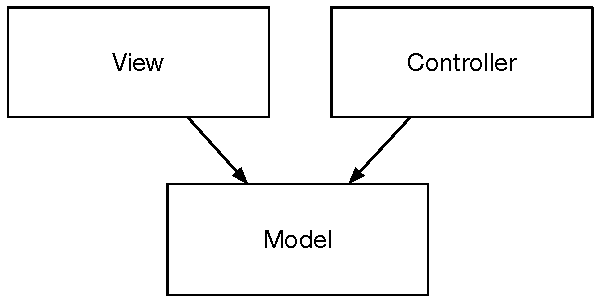
\includegraphics[height=4cm,keepaspectratio]{assets/concept/mvc_1.pdf}
    \caption{Classic MVC}
    \label{fig:mvc_1}
\end{figure}

\subsection{Modern MVC}

Modern MVC has evolved from being a software design pattern which handles components of an application to an architectural design pattern that defines the structure of an application itself. It has many similarities to the Layer Architecture. The responsibilities of each layer are slightly different to the typical presentation, business, and persistence layer definitions.

Most modern web frameworks such as Ruby on Rails, Symfony or the IOS environment refer to themselves as MVC based frameworks. The modern MVC concept has changed slightly. The component definitions are the same, but some responsibilities have shifted. Modern MVC strictly separates the model from the view. All modern frameworks state that the view should have as little logic as possible. Any logic implemented in the view should only be relevant to presentation. The view components should not directly reference the model components\cite{apple_MVC}\cite{symfony_MVC}.

\begin{figure}[H]
    \centering
    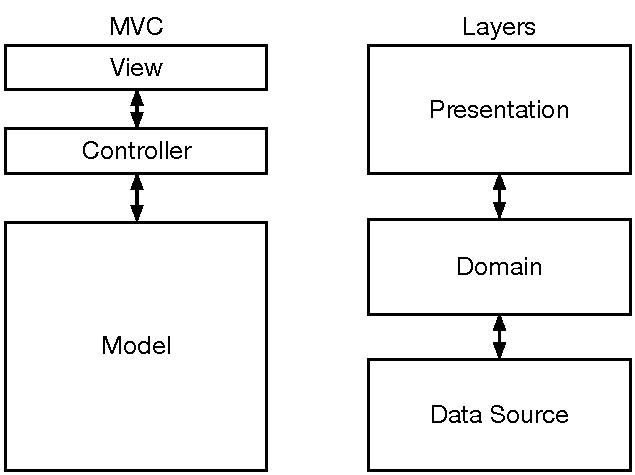
\includegraphics[height=4cm,keepaspectratio]{assets/concept/mvc_2.pdf}
    \caption{Modern MVC vs 3-Tier Layered Architecture}
    \label{fig:mvc_2}
\end{figure}

This division of responsibility has the added benefit of increased testability. GUIs are difficult to test, by removing as much logic as possible from the user interface there is less necessity to test it. The controller and model components can more easily be tested independently of one another using normal unit tests\cite{mvp_testing}.

\subsection{MVC Derivatives}

Many MVC derivatives exist. The main differences are where the division of responsibility is made and how it is labeled. MVVM defines a view model instead of a controller. The view model acts as a facade around the model and introduces a data binder element that is responsible for keeping the view and view model synchronised. The MVT, calls the view a template and the controller a view. The slight difference is that the template is basically a static file, with no logic, and placeholders for the data. The Django web framework uses this model, but there is little difference to the other MVC derivatives such as MVP ( model view presenter ). The AngularJS web framework takes ends the discussion of which design to follow by labelling itself a MVW ( model view whatever ) framework\cite{mvw}.


\begin{figure}[H]
    \centering
    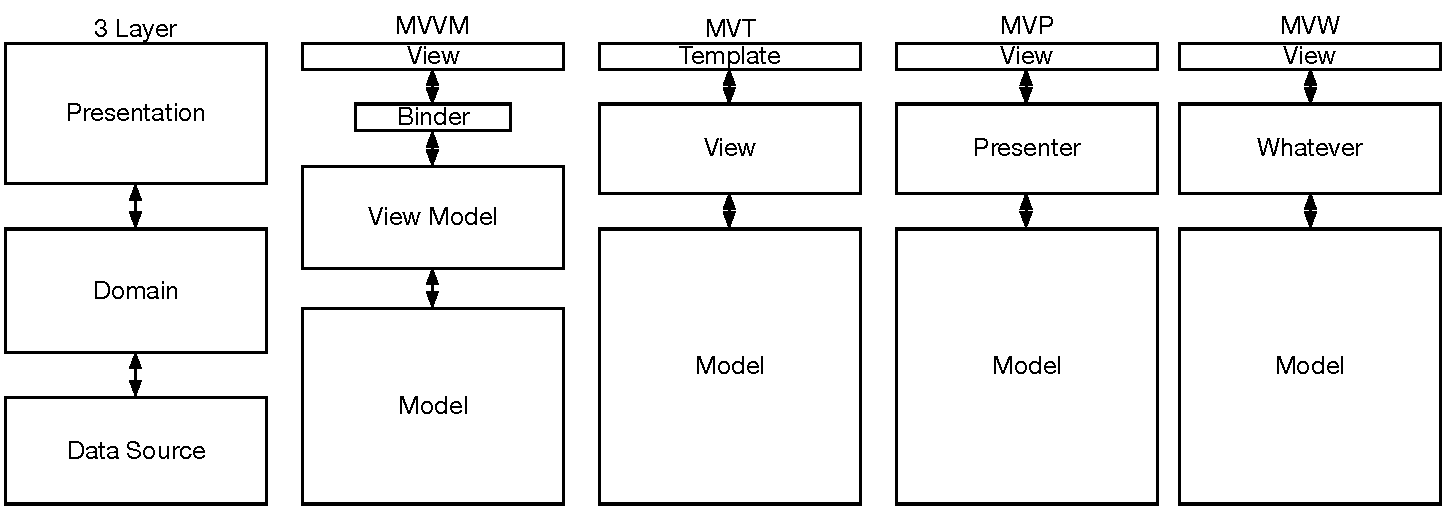
\includegraphics[height=4cm,keepaspectratio]{assets/concept/mvc_3.pdf}
    \caption{MVC Derivatives Overview}
    \label{fig:mvc_alt}
\end{figure}

\subsection{MVC and Smart Phone Applications}

Although most frameworks and environments targeted toward mobile application development use concepts from MVC, it can be difficult to define strict devision of responsibility, especially in conjunction with services provided from an online server. Often the responsibilities of the controller are reimplemented server side, some model management might occur in the app. Server and application code are developed using different languages and often most likely different developers. One solution is is to develop the app as a thin client, where it basically becomes the view component of MVC and the controllers and model are implemented on the server. Taken to the extreme, the app runs in a standard web browser and server provides the view components that emulate a native mobile user interface. This is referred to as a web app. Any logic in the view is implemented using javascript. Hardware support is limited to what the mobile browser provides access to. In order to extend hardware support a hybrid approach can be used in which the app implements a custom browser view which is extended with native capabilities. Here is division or responsibilities as defined by MVC become fuzzy. A fully native app working in conjunction with a web server will not conform well to the definitions of MVC.

\subsection{VIPER}

VIPER is a new software architecture pattern which extends MVC with some addition concepts that make it more adaptable to mobile applications, especially when they are extended with online server based services. The classic controller is split into a presenter and a controller, the model component is split into a central data manager communicating with many services and entities\cite{viper}.

\begin{figure}[H]
    \centering
    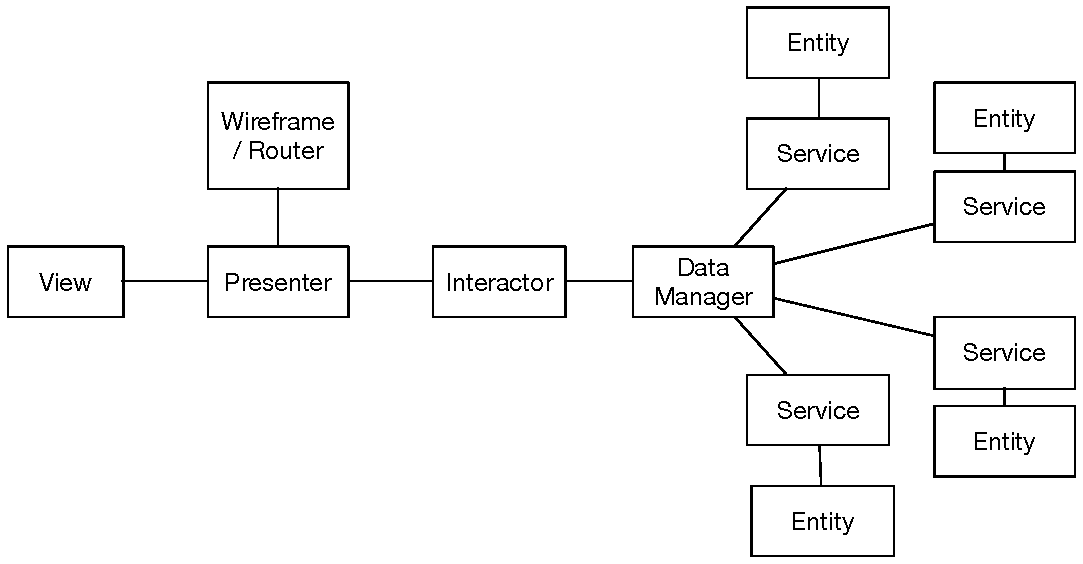
\includegraphics[height=6cm,keepaspectratio]{assets/concept/viper.pdf}
    \caption{VIPER Overview}
    \label{fig:viper}
\end{figure}

\begin{itemize}[label={}]

\item \textbf{View}: The view corresponds to the view as defined in modern MVC definitions, it is a slim component with as little logic as possible. It presents the current state of the models and provides “widgets” with which the user can interact.
\item \textbf{Presenter}: The presenter passes data to the view and handles events from the view. The presenter might perform some basic validation, in the case of a user sign-up scenario, for example, the presenter might validate that a user’s email is indeed formatted as a correct email, it will not validate if the email has already been used by someone else.

\item \textbf{Interactor}: Business logic is handled by the interactor. Most a what the model component in MVC was responsible for is handled here. The interactor however does not know anything about data storage, databases, or persistence. It does not know if data is local or accessible via a network.

\item \textbf{Data Manager}:
\item \textbf{Service}:
\item \textbf{Entity}:
\item \textbf{Wireframe / Router}:

\end{itemize}


\bibliography{references}{}
\bibliographystyle{plain}

\chapter{Appendix}

\chapter{Notes}
\section{Notes}

Research the medical app market:

\noindent
itunes store search api:

\begin{itemize}
\item official api :
\\ https://affiliate.itunes.apple.com/resources/documentation/itunes-store-web-service-search-api/
\\ limited to 200 results, no posibility to get next 200.
\item python wrapper
\\ https://github.com/ocelma/python-itunes
\\ too limited, better to use the python "requests" library
\\ still depends on official api so same limitations
\item rss feed with additional filters : https://rss.itunes.apple.com/us/?urlDesc=\%2Fgenerator
\\ can filter free or paid applications, can rank by user feedback and gross

\end{itemize}

\noindent
android seach api:
\begin{itemize}
\item no official api
\item unofficial : https://github.com/egirault/googleplay-api
\\ hackey, pretends to be an android device
\end{itemize}

\noindent
FDA (U.S. Food and Drug Administration) Mobile Medical App Submissions
\begin{itemize}
\item API : https://open.fda.gov/device/510k/ example : https://api.fda.gov/device/510k.json?limit=20\&search=tumor\%20skin\%20app
\item reference : https://open.fda.gov/device/510k/reference/
\\ API is useable but might have too much information (not just for mobile apps).
\\ I need to reasearch if there are adequate filtering possibilities to narrow down results
\end{itemize}

\noindent
\begin{itemize}
\item A
\item B
\end{itemize}



\end{document}